\documentclass[beamer=true]{standalone}
\usepackage{../../preamblesnotes}

% \includeonlylecture{thirdChapter}
\begin{document}
\settitle{波動現象Phenomena of wave motion}{波動學第二課}{周末班}

\lecture{First lecture}{firstChapter}
\begin{frame}{連續機械行波的能量分佈Distribution of energies in continuous waves}
    \begin{block}{考慮某一瞬間各質點的能量/單一質點隨時間推移的能量:}
        \begin{itemize}
            \item 質點的總機械能Total mechanical energy of a particle = 動能KE + 勢能PE
                  \begin{itemize}
                      \item 總機械能:跟振幅相關。($\propto A^2$)
                            \\ Total mechanical energy: related to amplitude. ($\propto A^2$)
                      \item 勢能:跟位移相關。($\propto y^2$)
                            \\ Potential energy: related to displacement of a particle.($\propto y^2$)
                      \item 動能:跟質點的移動速率相關。($\propto v^2$)
                            \\ Kinetic energy: related to speed of a particle.($\propto v^2$)
                  \end{itemize}
            \item 若沒有能量損耗,總機械能不變。
                  \\ When there is no energy loss, total mechanical energy remains the same.
        \end{itemize}
    \end{block}
\end{frame}


\begin{frame}{連續機械行波的能量分佈Distribution of energies in continuous waves}
    \par{\par\centering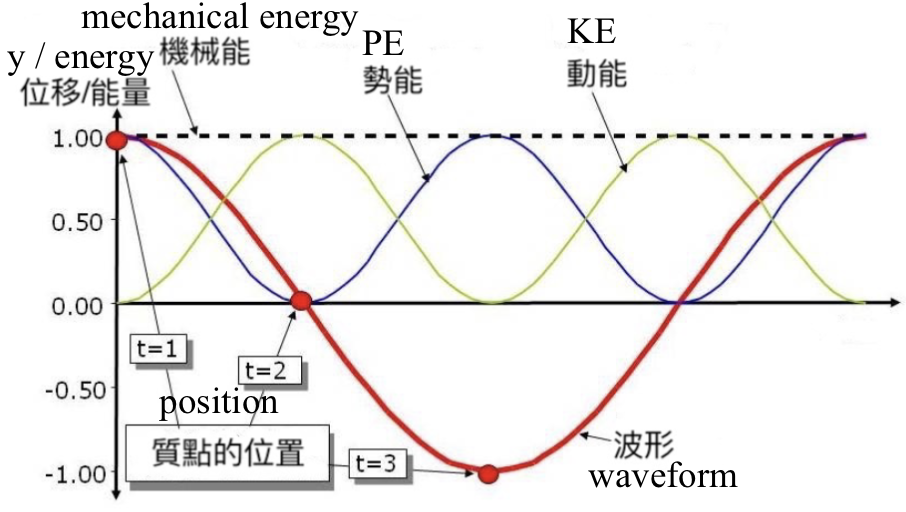
\includegraphics[width=\textwidth]{./img/ch2_cf_2024-05-22-11-31-38.png}\par}

\end{frame}

\begin{frame}[t]{}
    圖(a)顯示九個均勻分佈的質點。圖(b)顯示一縱波各質點的位置。在此時此刻,下列哪線圖正確地顯示各點的勢能PE隨位置x的變化?\\Figure (a) shows nine uniformly distributed particles. Figure (b) displays the positions of the particles in a longitudinal wave. At this moment, which of the following graphs accurately represents the variation of potential energy (PE) with respect to the position (x) of each point?
    \begin{figure}
        \centering
        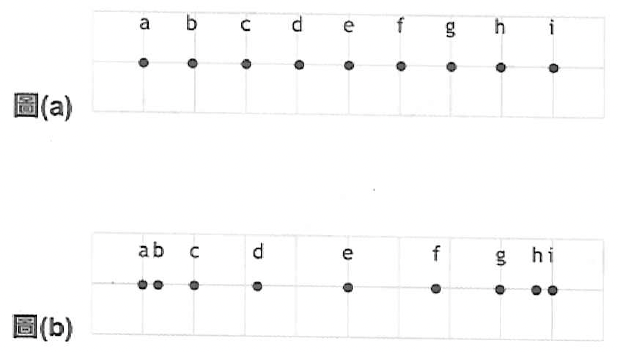
\includegraphics[width=0.7\linewidth]{images/Screenshot 2023-09-27 at 8.21.03 AM.png}


    \end{figure}

\end{frame}

\begin{frame}{}
    \noindent\begin{tasks}%(2)[item-indent=2em,label-offset=2em,label-width=1em,column-sep=0pt]
        \task \topalign{
            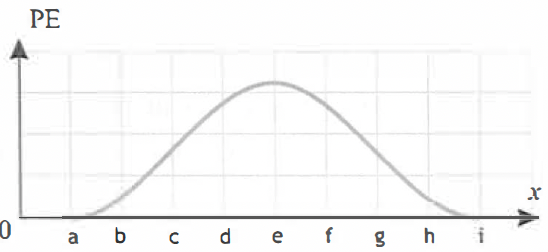
\includegraphics[width=.43\linewidth]{images/Screenshot 2023-09-27 at 8.30.49 AM.png}

        }
        \task \topalign{    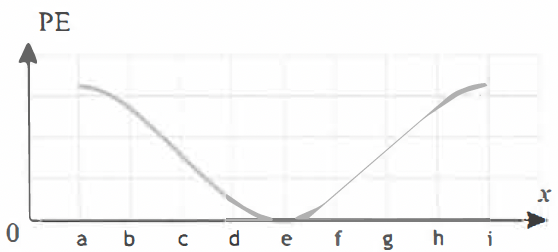
\includegraphics[width=.43\linewidth]{images/Screenshot 2023-09-27 at 8.30.55 AM.png}
        }
        \task \topalign{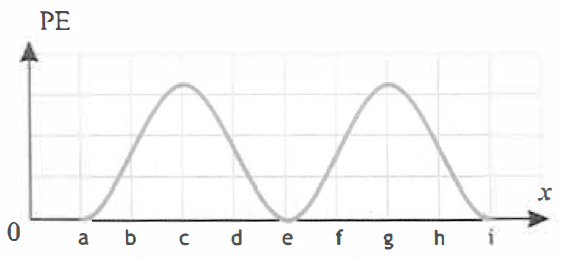
\includegraphics[width=.43\linewidth]{images/Screenshot 2023-09-27 at 8.31.00 AM.png}}

        \task \topalign{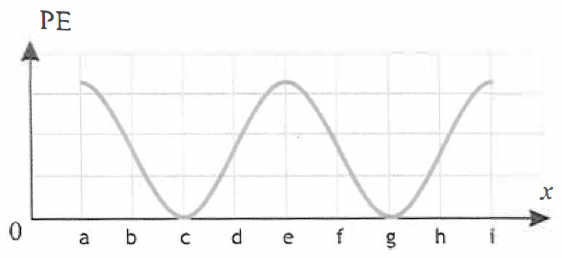
\includegraphics[width=.43\linewidth]{images/Screenshot 2023-09-27 at 8.31.03 AM.png}}

    \end{tasks}
\end{frame}




\begin{frame}{水波槽ripple tank}
    \begin{figure}
        \centering
        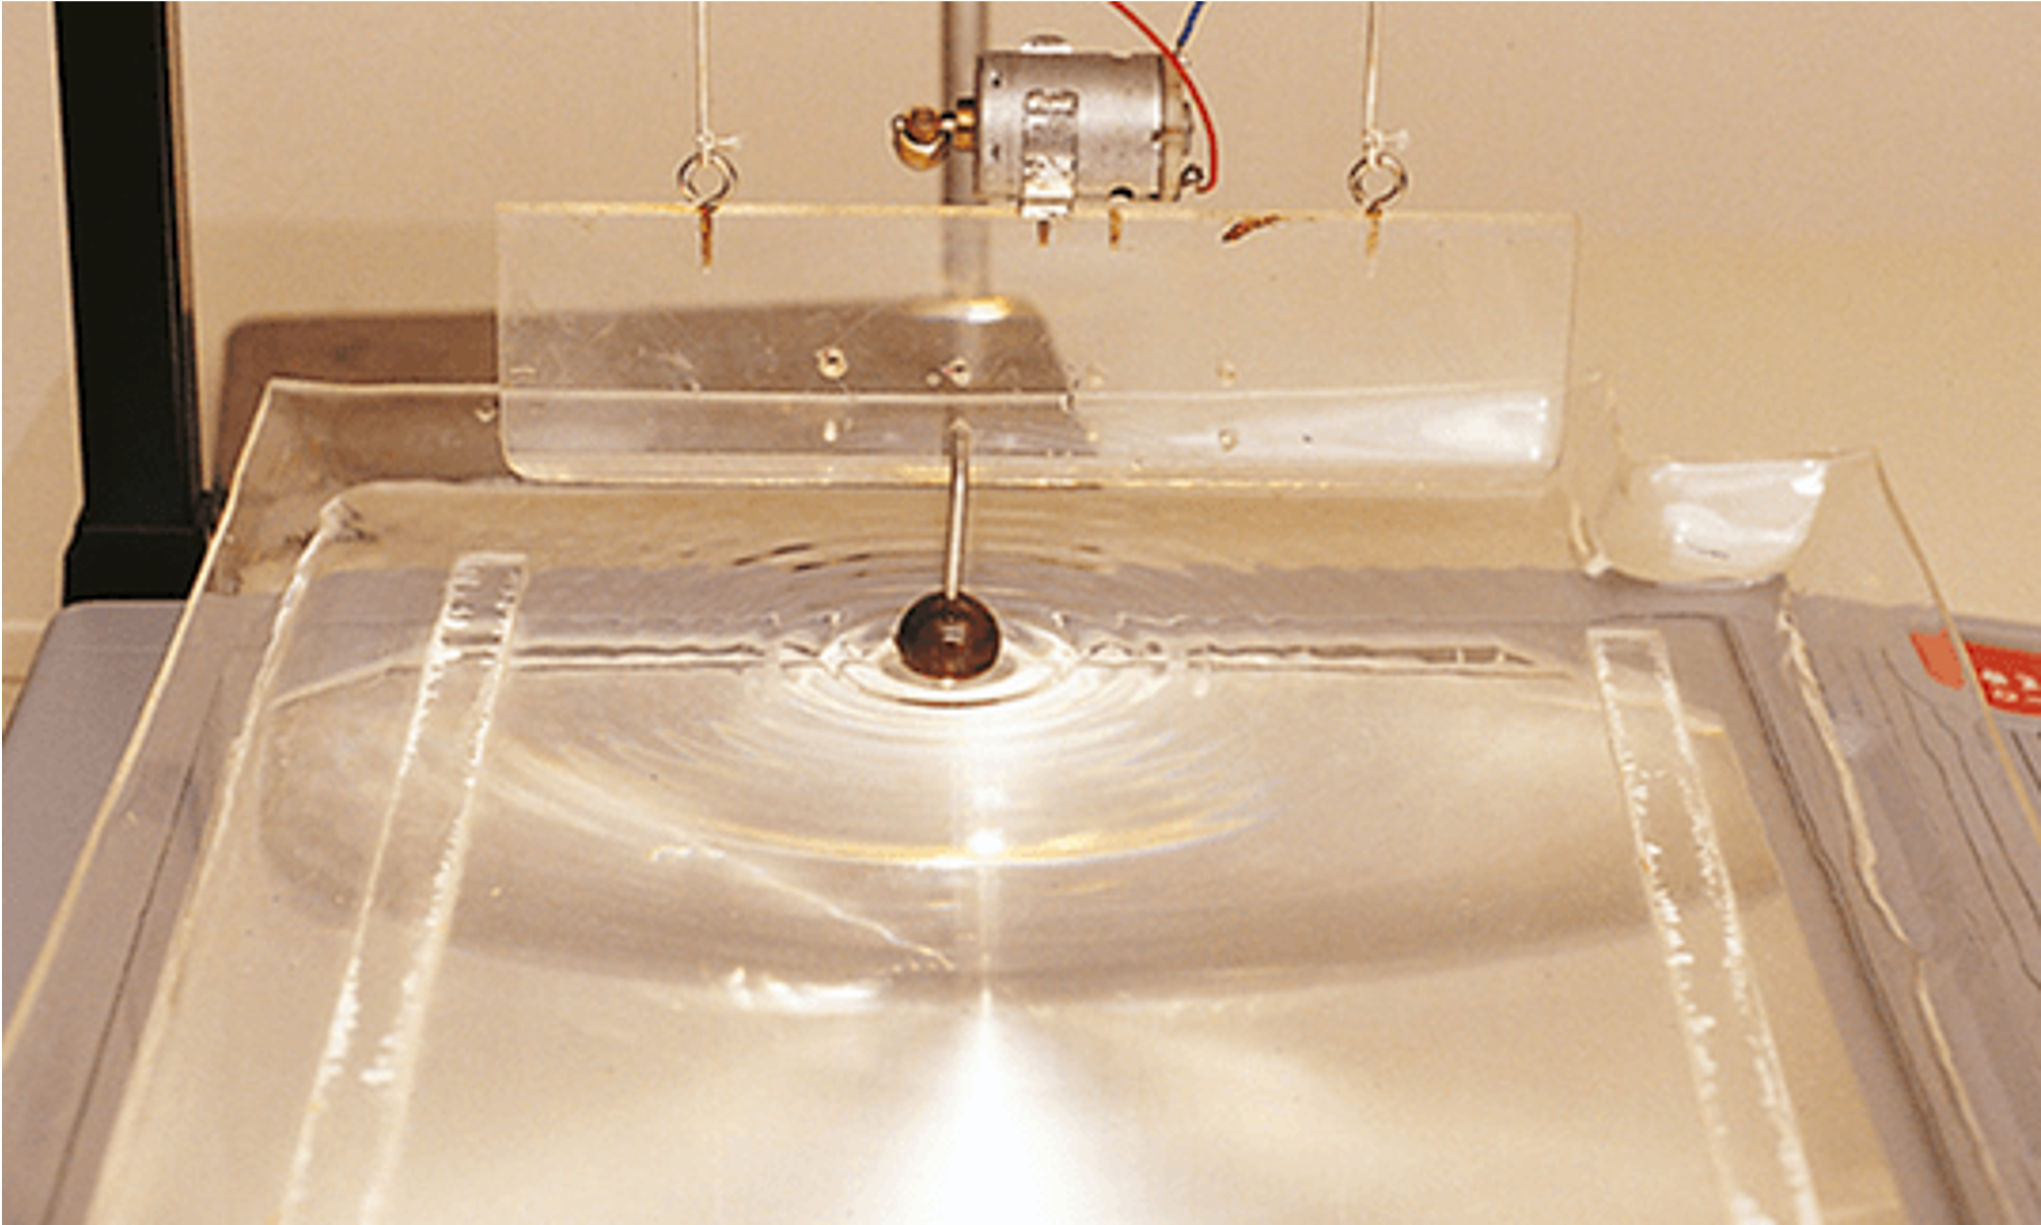
\includegraphics[width=0.5\linewidth]{images/Picture 1.png}
        \caption{水波槽可以用來產生水波ripple tanks can be used to produce water wave}

    \end{figure}
\end{frame}




\begin{frame}{水波的傳播Propagation of water wave}
    \begin{itemize}
        \item 當點振源移動一次上下一個完整的周期時,會產生一個完整的水波波長。\\When point source completes one full oscillation, one wavelength of wave is produced.
              \begin{itemize}
                  \item 點振源的頻率=水波的頻率。\\frequency of point source = frequency of water wave.
                  \item 點振源無法控制水波的速率。\\ point source cannot control speed of water wave.
                  \item $\because v=f\ \lambda$,頻率越大,波長越短。\\$\because v=f\ \lambda$, wavelength decreases as frequency increases.
              \end{itemize}
    \end{itemize}
    % \begin{figure}
    %     \centering
    %     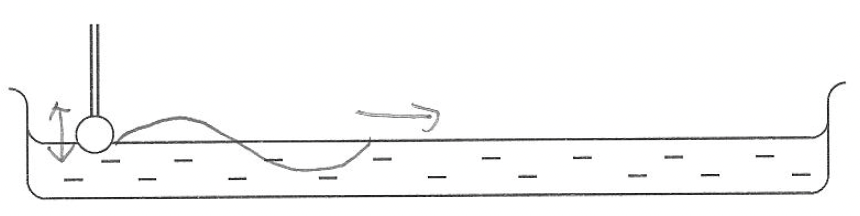
\includegraphics[width=0.5\linewidth]{images/Screenshot 2023-09-25 at 2.25.17 AM.png}
    %     % \caption{水波槽可以用來}
    % \end{figure}
    % \par{\par\centering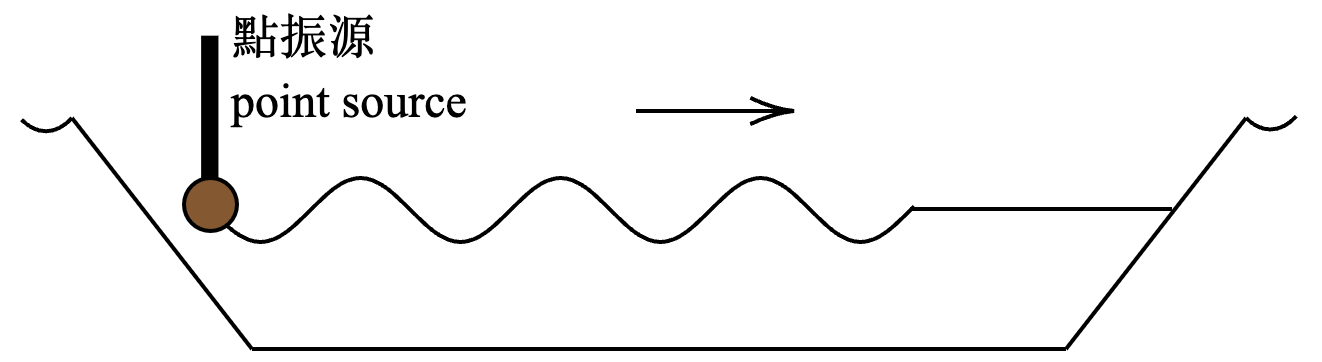
\includegraphics[width=.6\textwidth]{./img/ch2_cf_2024-05-24-13-18-05.png}\par}
    \par{\par\centering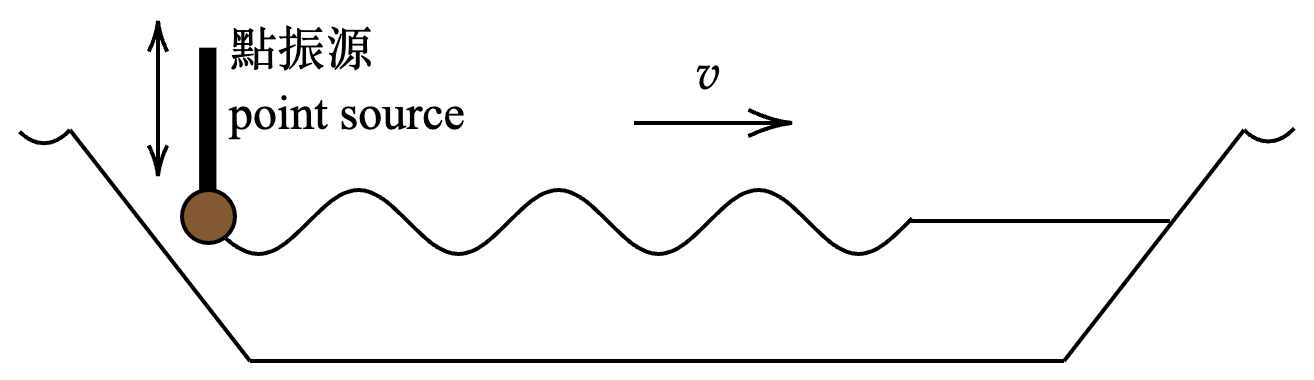
\includegraphics[width=.6\textwidth]{./img/ch2_cf_2024-05-24-13-19-18.png}\par}
\end{frame}

\begin{frame}{製造水波Generating water wave}
    \begin{columns}
        \column{.5\textwidth}
        \begin{figure}
            \centering
            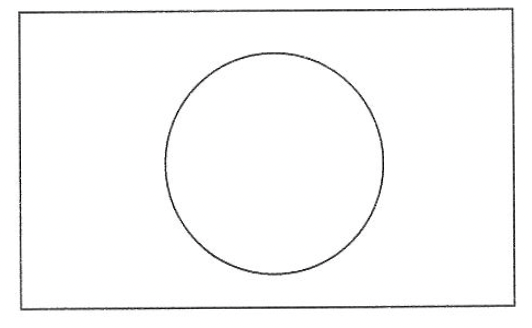
\includegraphics[width=0.97\linewidth]{images/Screenshot 2023-09-25 at 2.30.30 AM.png}
            \caption{脈衝水波 a pulse of water wave}

        \end{figure}
        \column{.5\textwidth}
        \begin{figure}
            \centering
            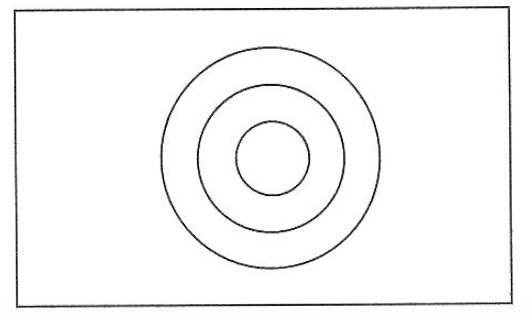
\includegraphics[width=1\linewidth]{images/Screenshot 2023-09-25 at 2.31.45 AM.png}
            \caption{連續水波 continuous water wave}

        \end{figure}
    \end{columns}
\end{frame}



\begin{frame}{以不同角度觀察水波 observe water waves}
    % \begin{figure}
    %     \centering
    %     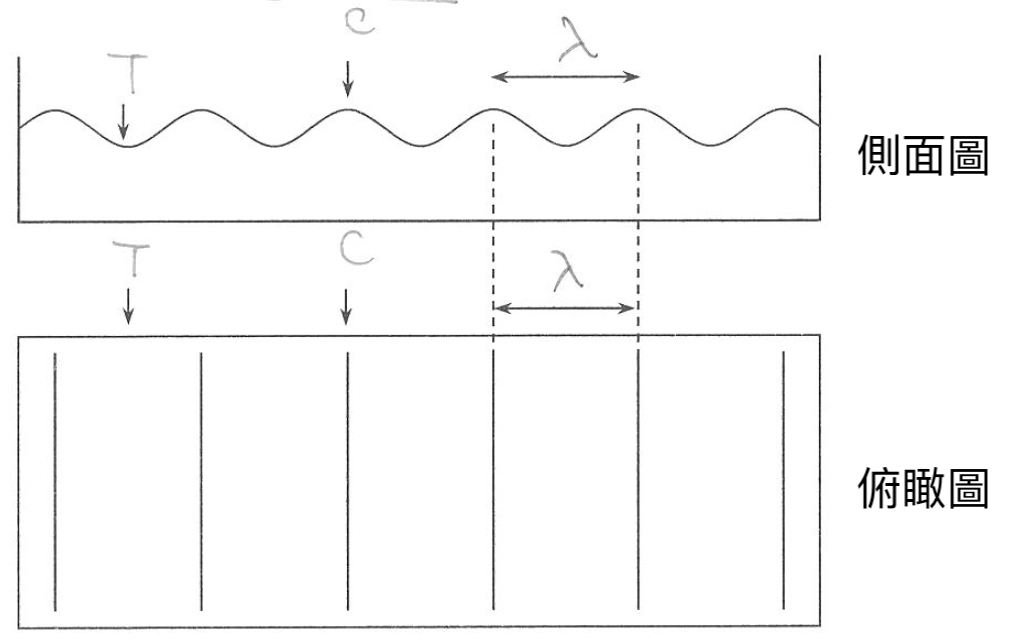
\includegraphics[width=1\linewidth]{images/Screenshot 2023-09-25 at 2.33.31 AM.png}


    % \end{figure}
    \par{\par\centering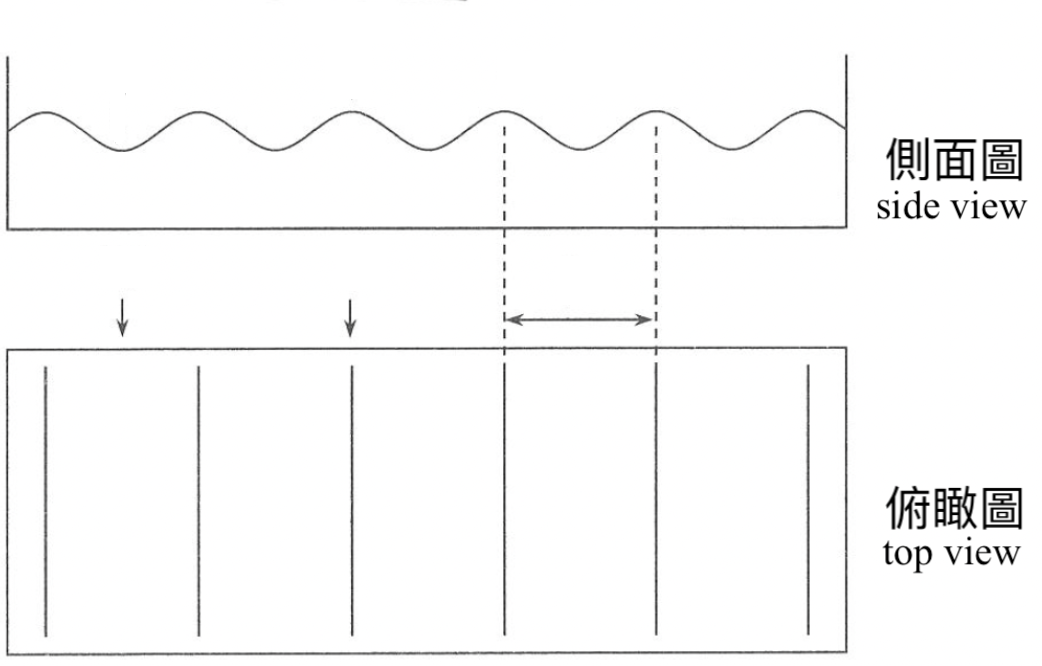
\includegraphics[width=\textwidth]{./img/ch2_cf_2024-05-24-13-08-21.png}\par}
\end{frame}


\begin{frame}{在屏幕上形成的條紋 water wave formed on a screen}
    \begin{figure}
        \centering
        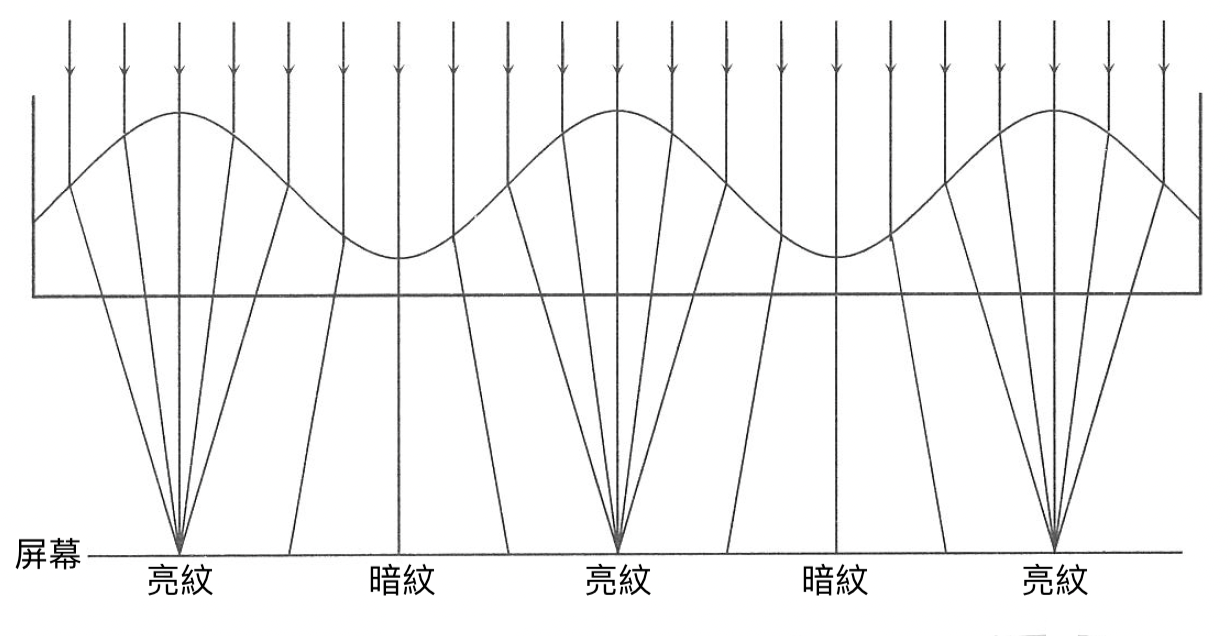
\includegraphics[width=0.75\linewidth]{images/Screenshot 2023-09-26 at 9.55.36 PM.png}
    \end{figure}
    \begin{itemize}
        \item 波峰聚焦光線形成光紋。\\Crests converge light rays and form bright fringes.
        \item 波谷發散光線形成暗紋。\\Troughs diverge  light rays and form dark fringes.
    \end{itemize}
\end{frame}


\begin{frame}{波陣面和射線Wavefront and rays}
    \begin{itemize}
        \item 波峰連接的線稱為波陣面。\\Wavefront: line connecting neighboring crests particles particles.
              % \item 在同一波陣面上,所有質點都以同相振動。\\On the same wavefront, all particles vibrate in-phase.
        \item 射線:表示波的傳播方向的線\\Ray: lines showing direction of travel of waves.
        \item 波陣面必定垂直於射線。\\Wavefront must be perpendicular to rays.
    \end{itemize}\bigskip
    \begin{columns}
        \column{.5\textwidth}
        \begin{figure}
            \centering
            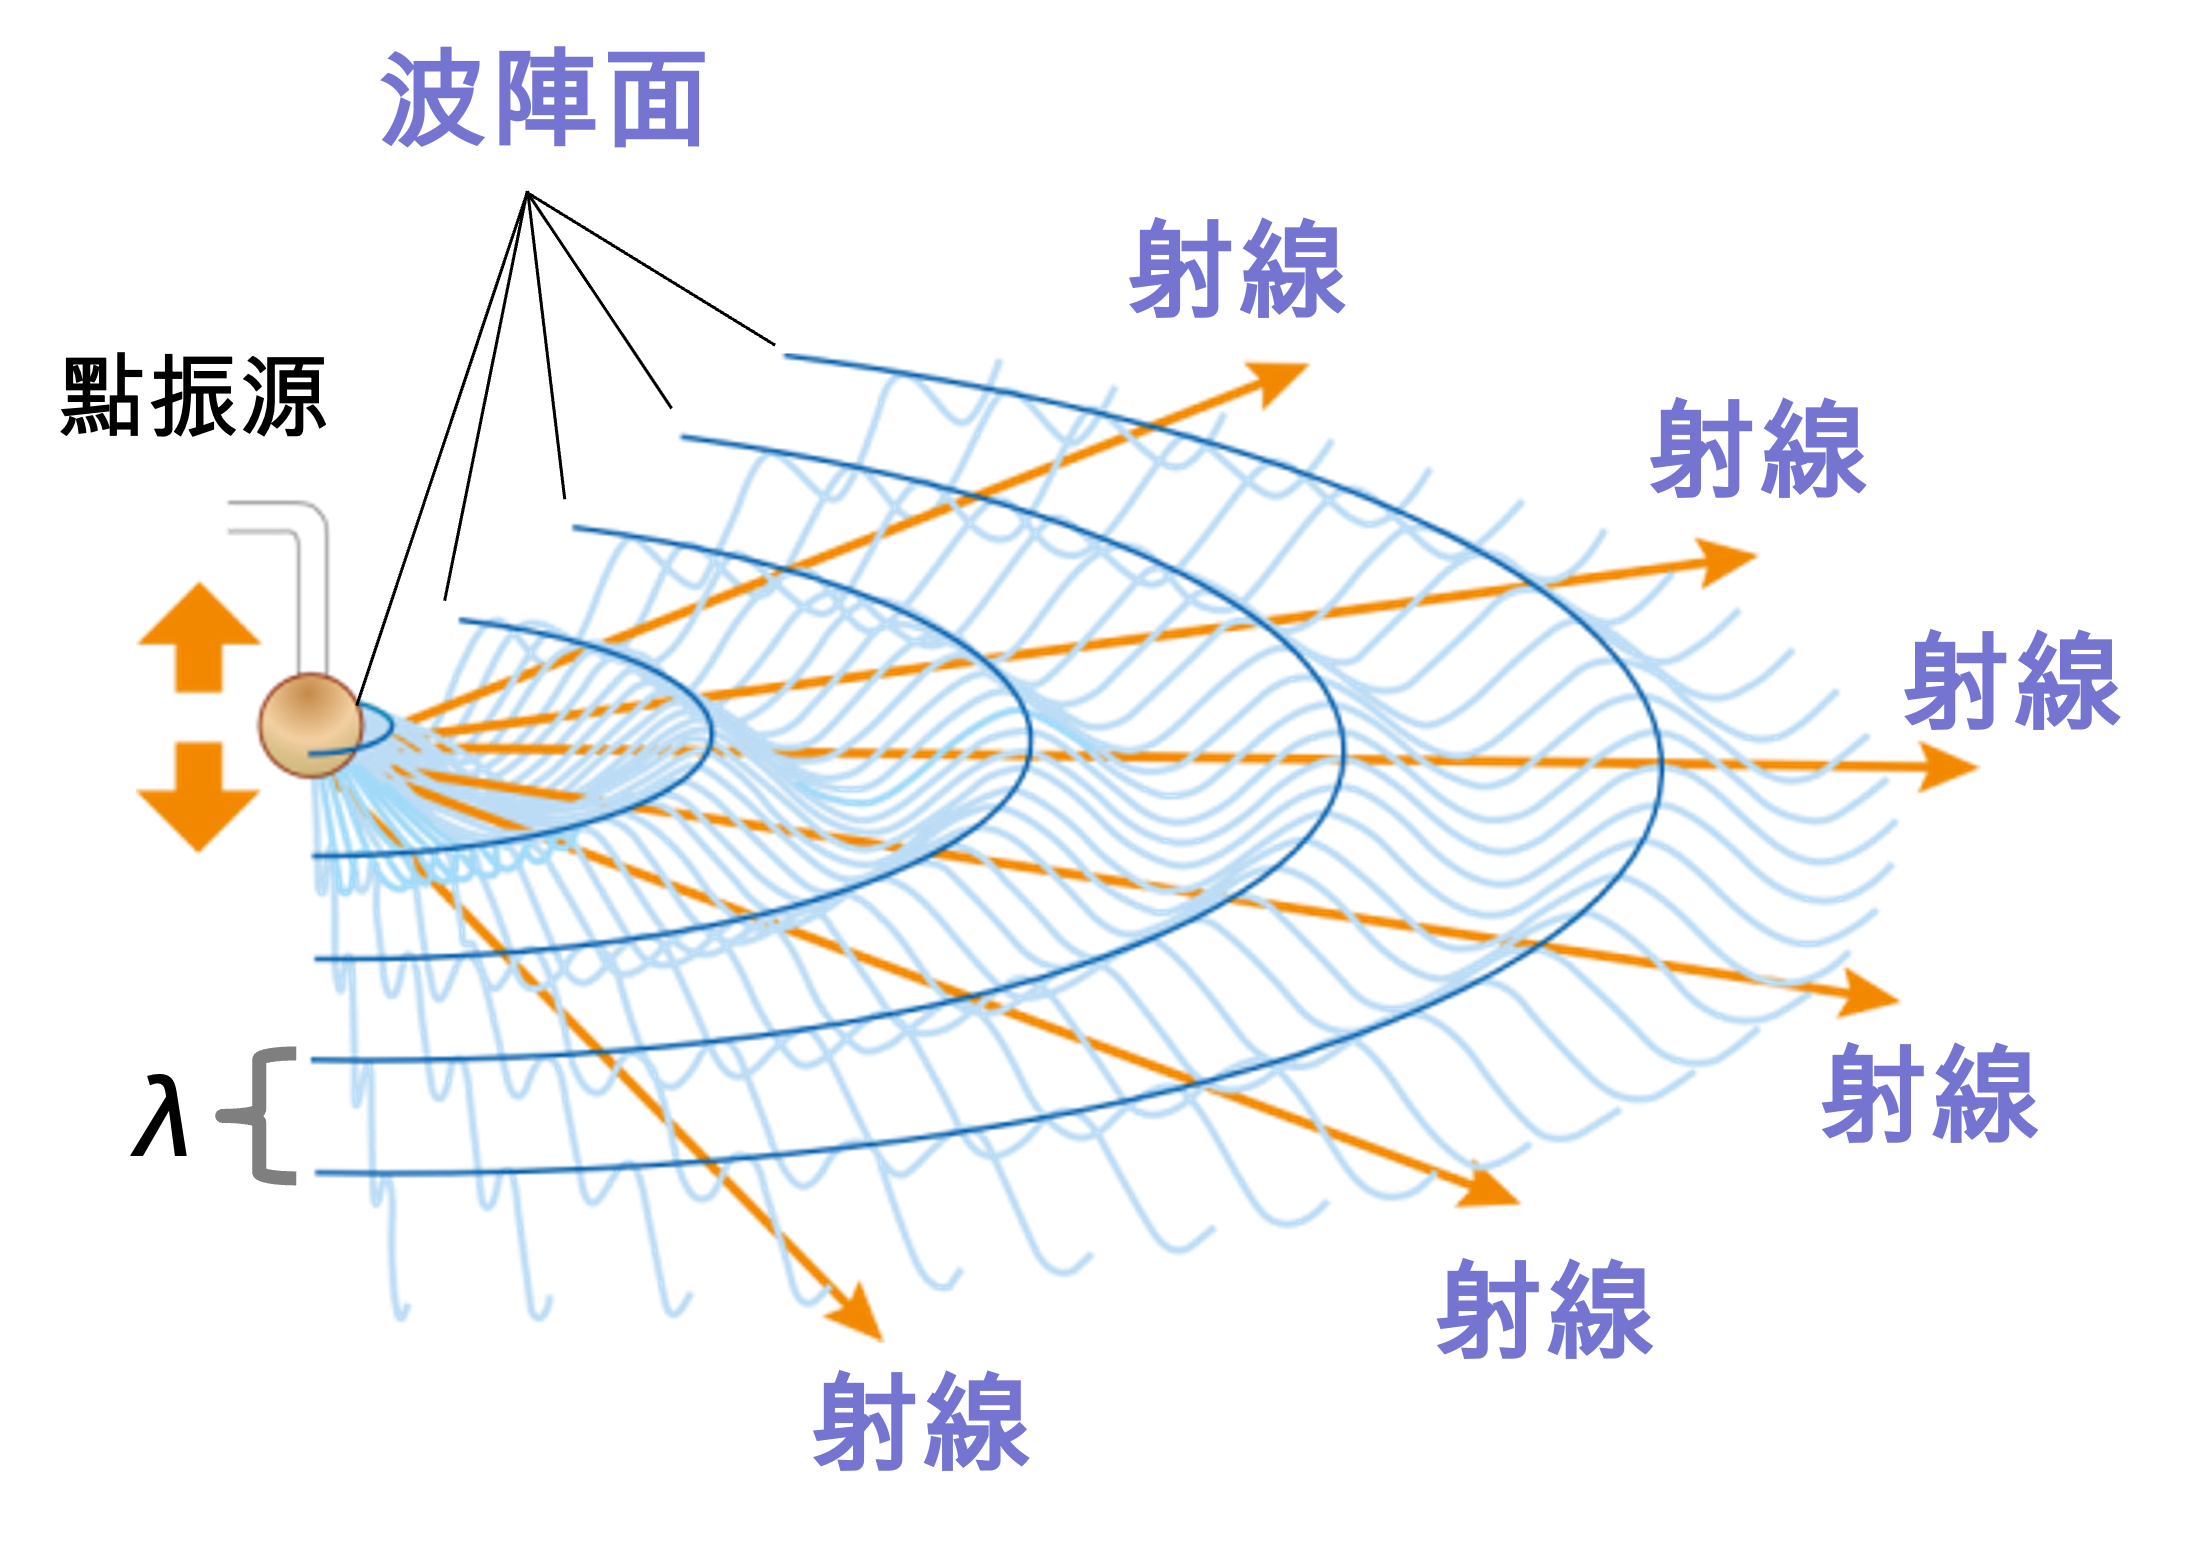
\includegraphics[width=\linewidth]{images/1}
            % \caption{點振源產生圓形波陣面}

        \end{figure}

        \column{.5\textwidth}
        % \begin{figure}
        %     \centering
        %     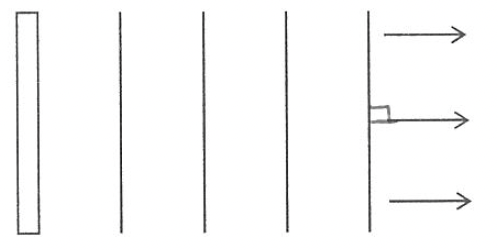
\includegraphics[width=1\linewidth]{images/Screenshot 2023-09-25 at 2.39.25 AM.png}
        %     \caption{直振源產生直線波陣面}

        % \end{figure}
        \begin{figure}
            \centering
            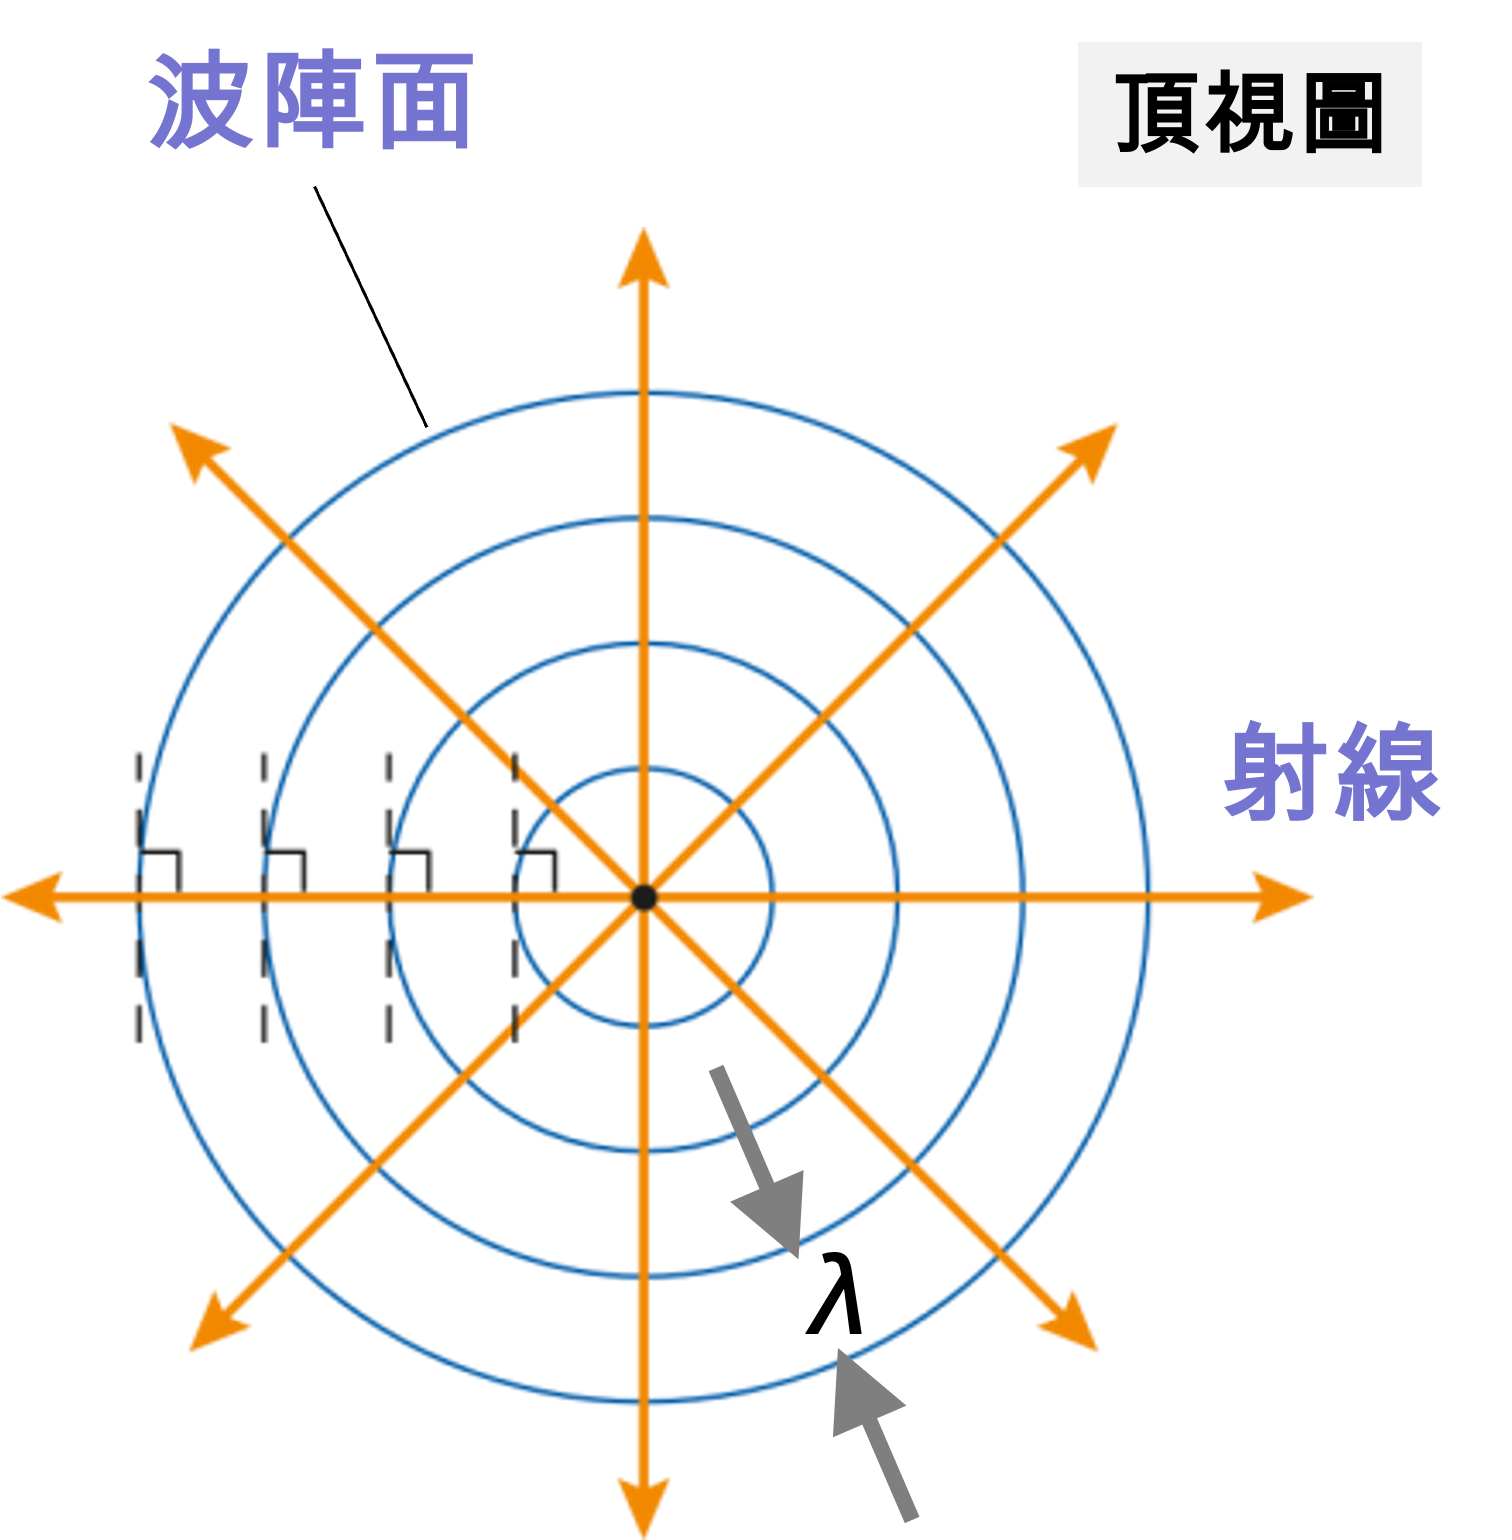
\includegraphics[width=0.7\linewidth]{images/2.png}
            % \caption{點振源產生圓形波陣面}

        \end{figure}
        % \begin{figure}
        %     \centering
        %     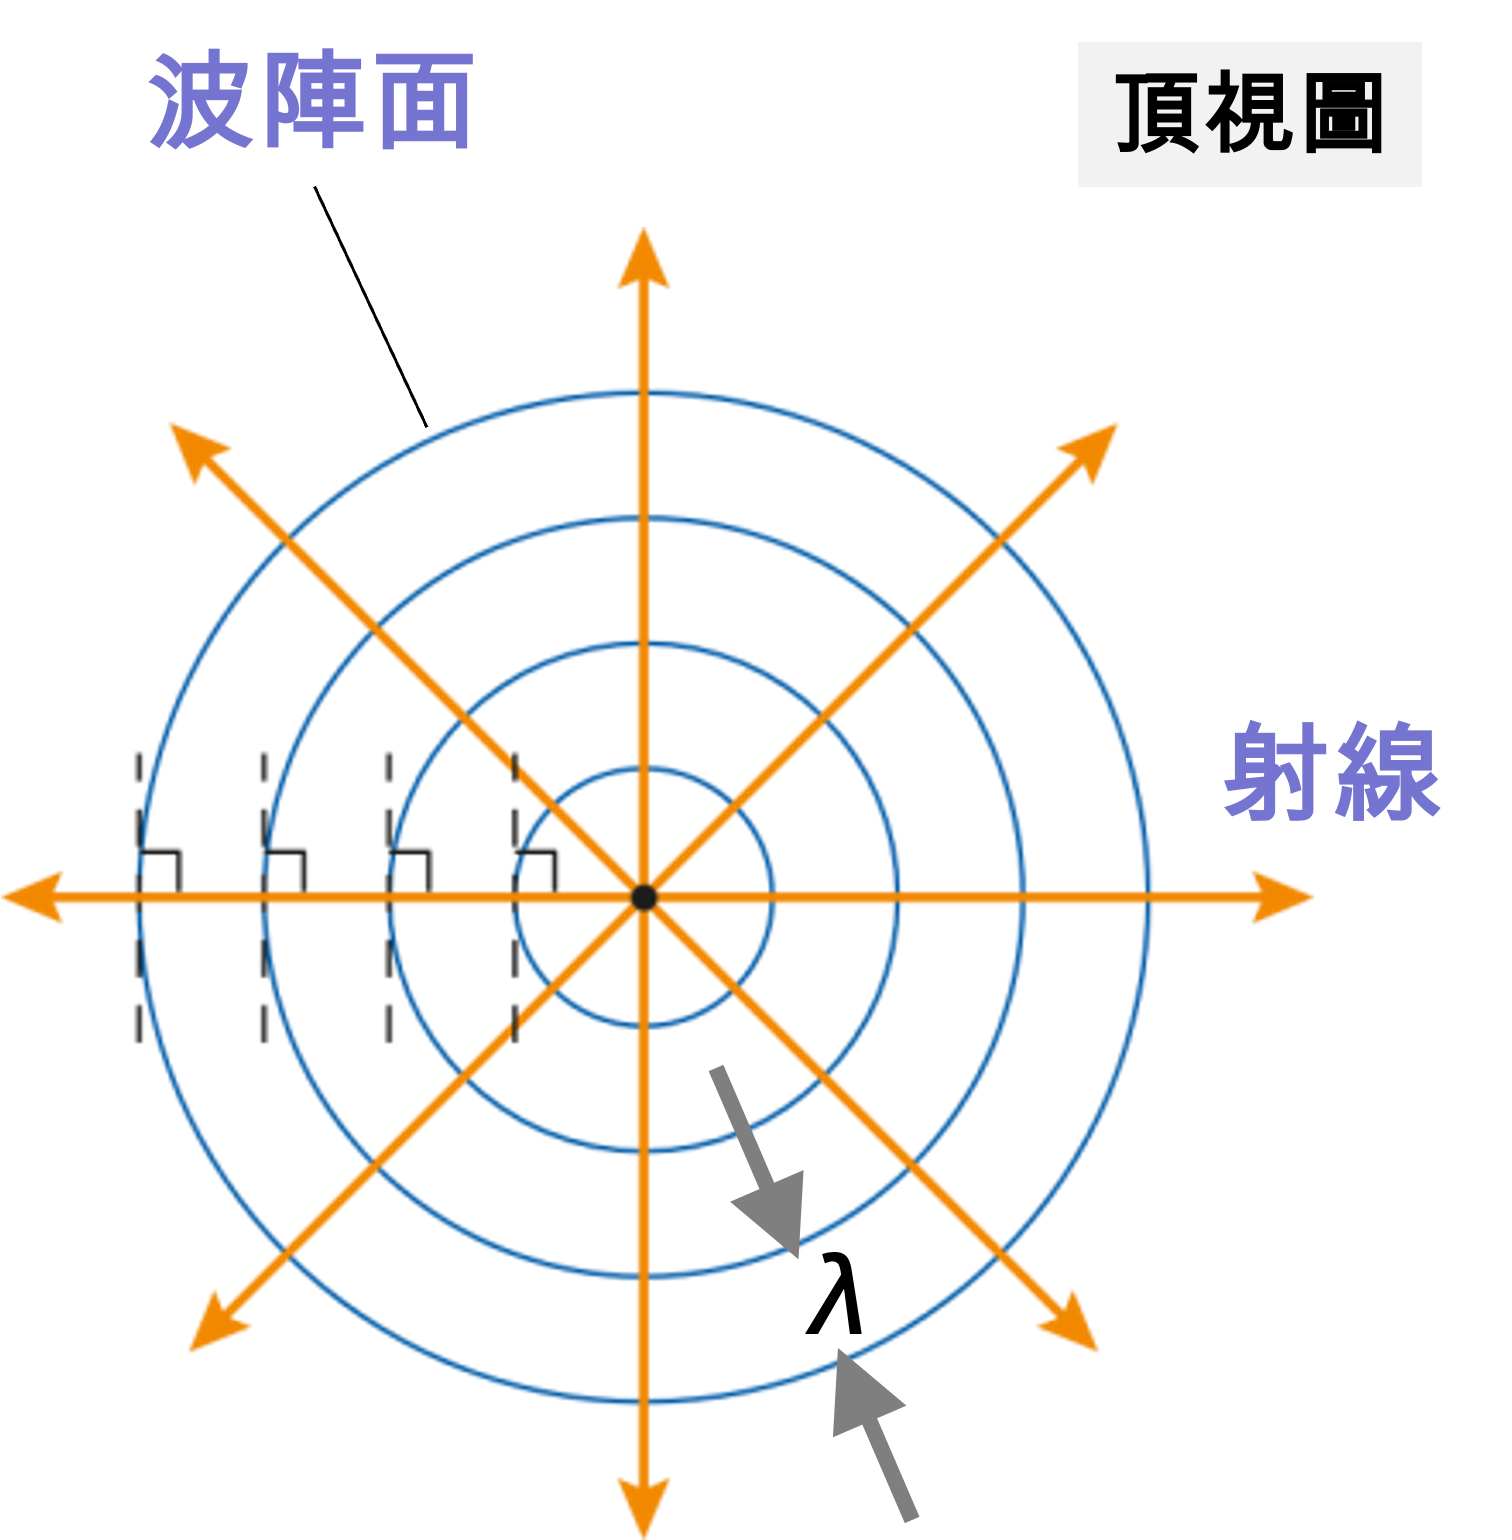
\includegraphics[width=1\linewidth]{images/2.png}


        % \end{figure}
    \end{columns}
\end{frame}

\begin{frame}{波陣面和射線Wavefront and rays}
    \begin{columns}
        \column{.5\textwidth}
        \begin{figure}
            \centering
            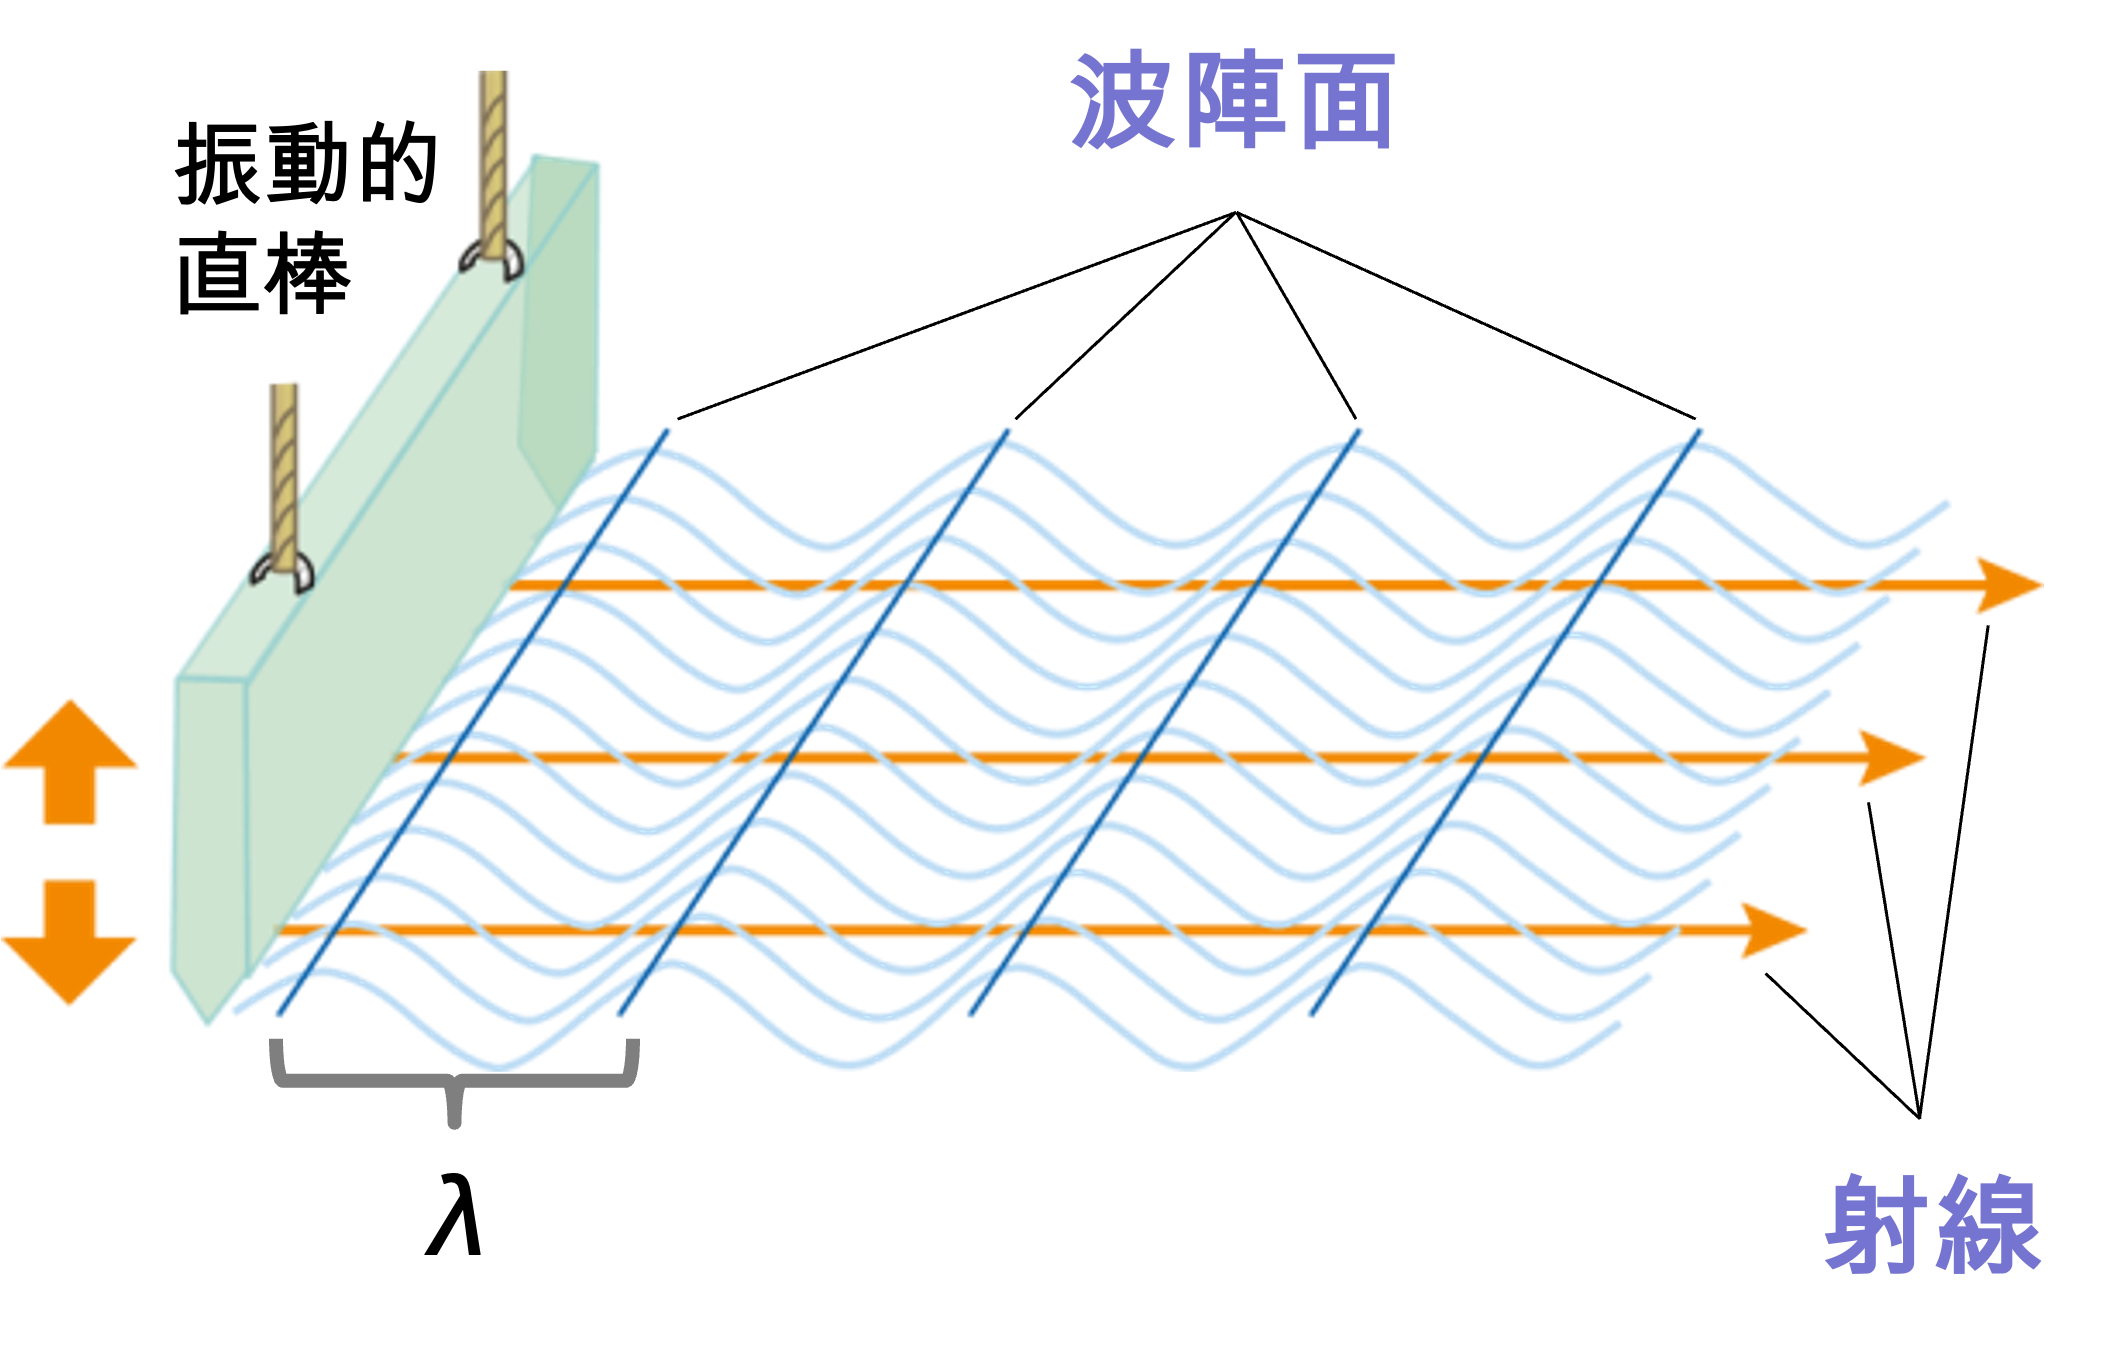
\includegraphics[width=1\linewidth]{images/3.png}


        \end{figure}
        \column{.5\textwidth}
        % \begin{figure}
        %     \centering
        %     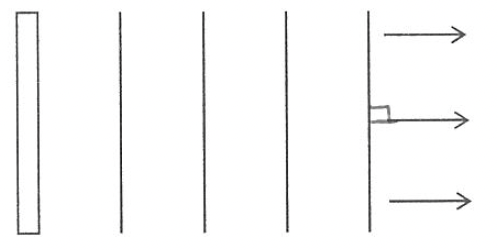
\includegraphics[width=1\linewidth]{images/Screenshot 2023-09-25 at 2.39.25 AM.png}
        %     \caption{直振源產生直線波陣面}

        % \end{figure}
        \begin{figure}
            \centering
            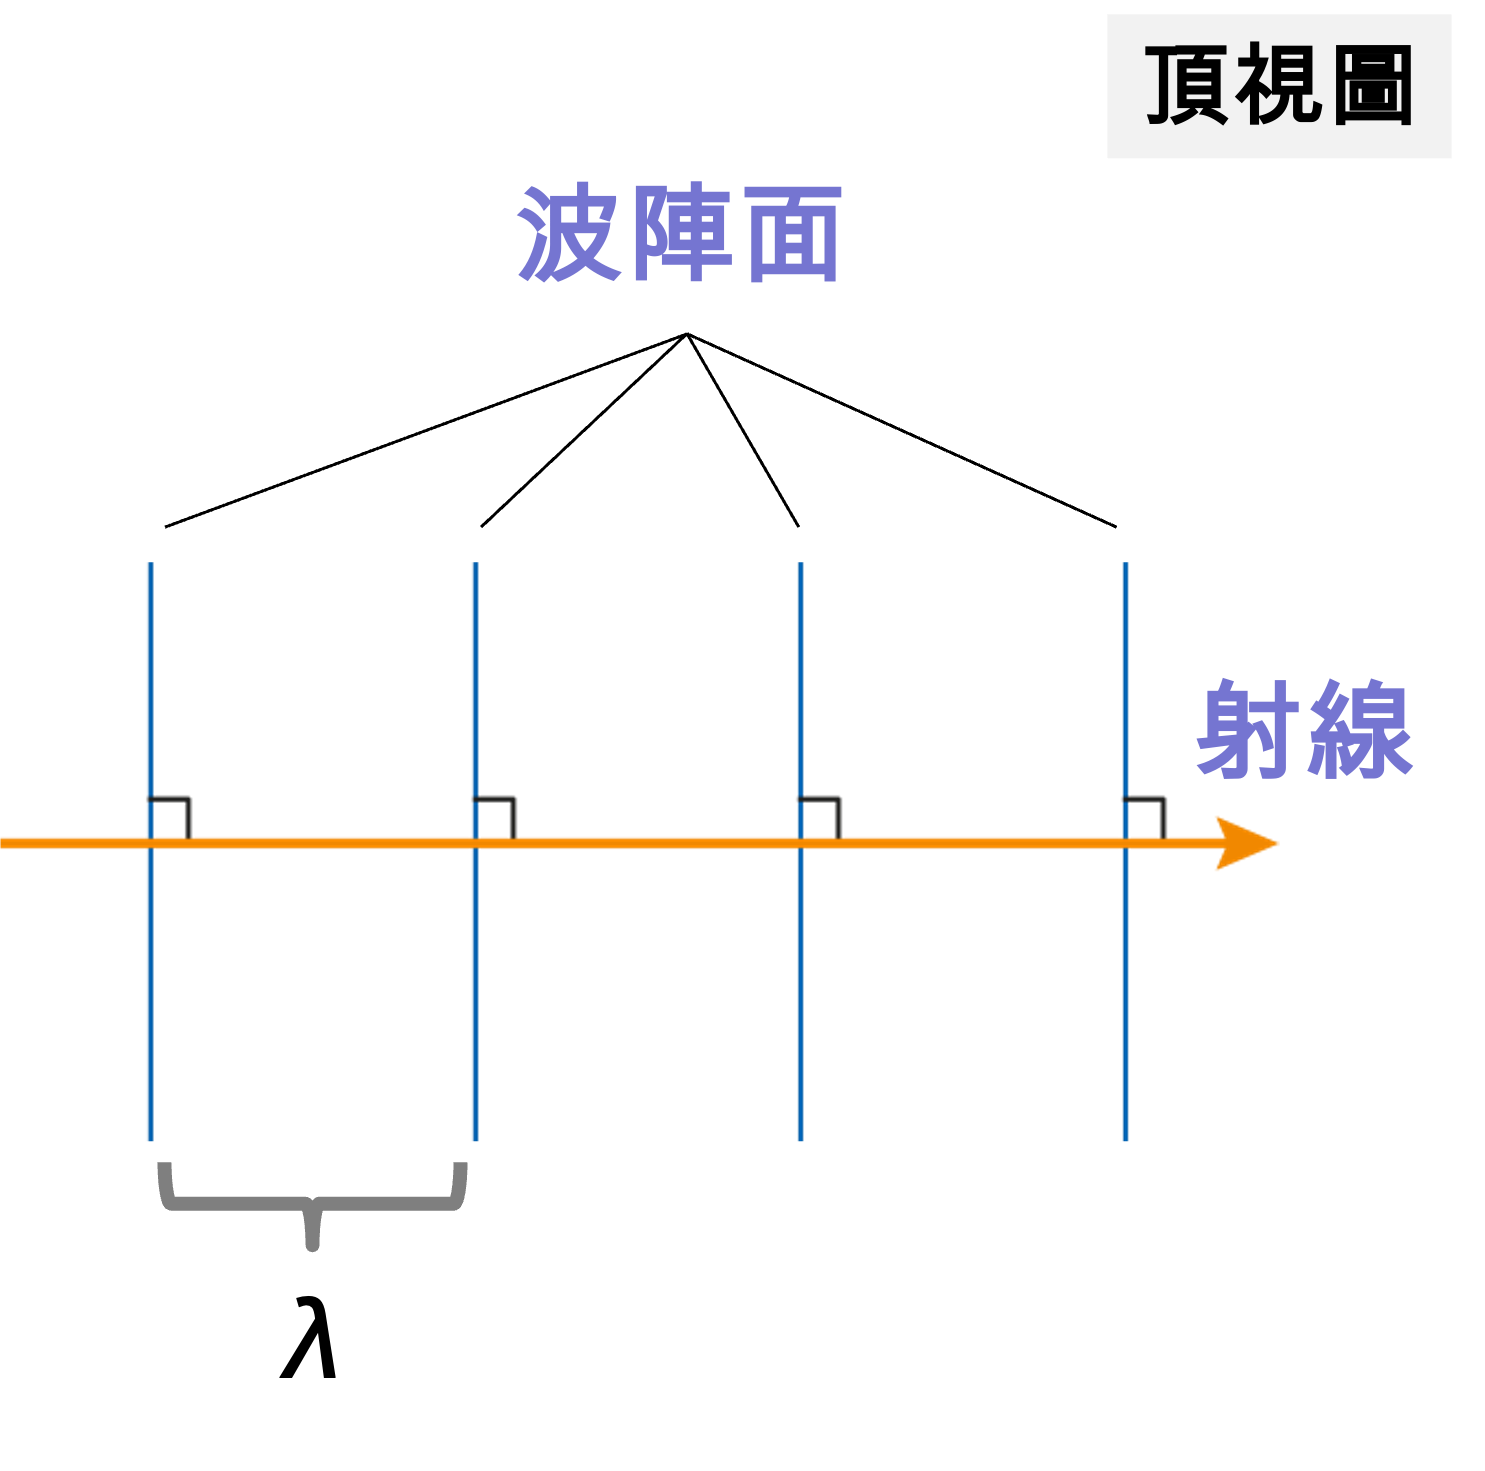
\includegraphics[width=1\linewidth]{images/4.png}


        \end{figure}
        % \begin{figure}
        %     \centering
        %     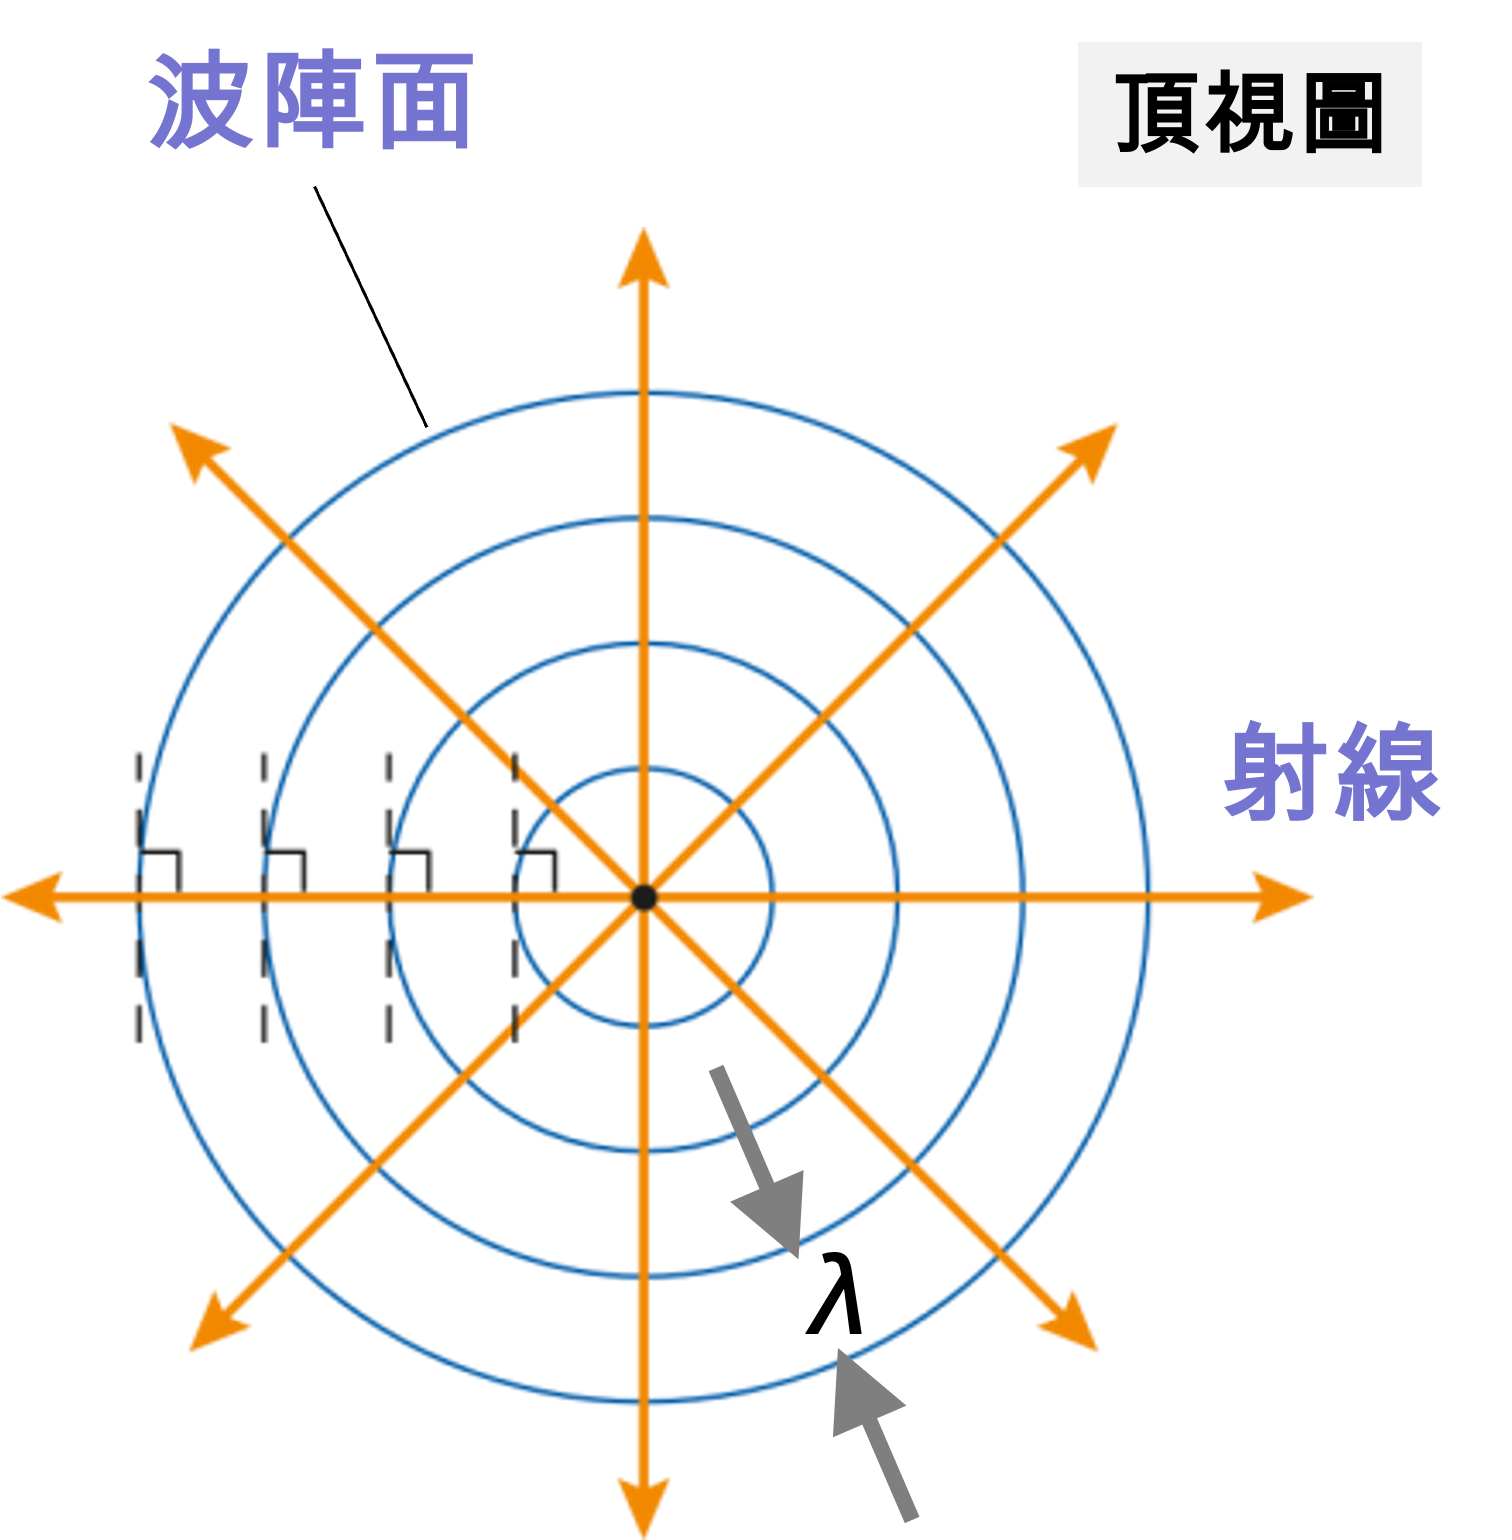
\includegraphics[width=1\linewidth]{images/2.png}


        % \end{figure}
    \end{columns}
\end{frame}

\begin{frame}[t]{例題Example}
    左圖和右圖分別是兩個直線水波P和Q。其中P的水比較淺。比較兩波的\(\lambda,v,f\)。\\The left and right figures respectively depict two straight water waves, labeled as P and Q. Wave P is shallower. Compare \(\lambda,v,f\) of the two waves.
    \begin{figure}
        \centering
        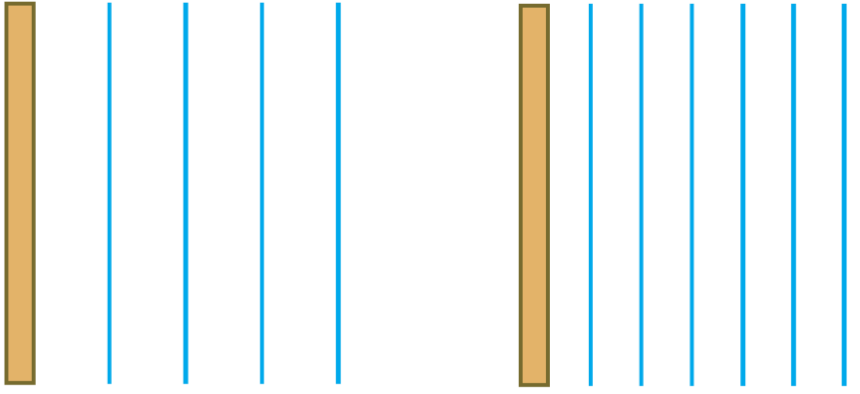
\includegraphics[width=0.65\linewidth]{images/Screenshot 2023-09-26 at 11.25.42 PM.png}


    \end{figure}
\end{frame}

\begin{frame}{量度水波的頻率Measuring frequency of water wave}
    \begin{itemize}
        \item 在黑暗的環境下,調整頻閃觀察器的頻率直至波形看起來靜止不動。\\In dim environment, adjust a stroboscope so that a frozen wave pattern is observed.
        \item 這時頻閃觀察器的頻率=波的頻率。\\Frequency of stroboscope = frequency of wave.

    \end{itemize}\bigskip
    \begin{columns}
        \column{.5\textwidth}
        \begin{figure}
            \centering
            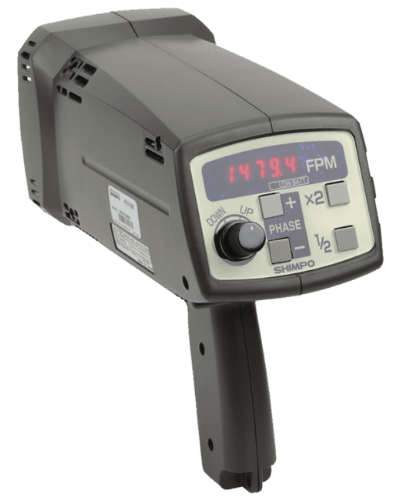
\includegraphics[width=0.6\linewidth]{images/Screenshot 2023-09-26 at 10.05.09 PM.png}


        \end{figure}
        \column{.5\textwidth}
        \begin{figure}
            \centering
            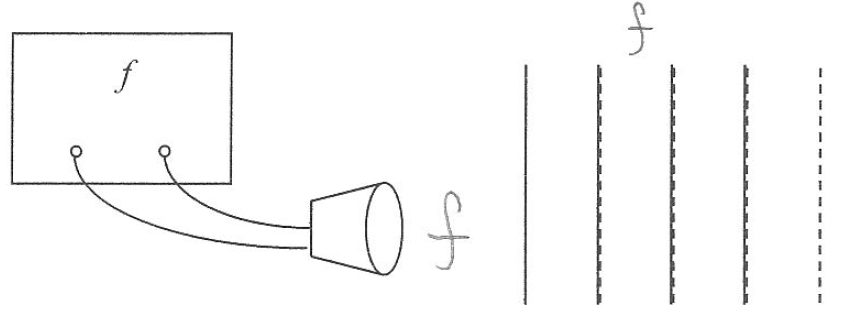
\includegraphics[width=1\linewidth]{images/Screenshot 2023-09-26 at 10.08.47 PM.png}


        \end{figure}
    \end{columns}
\end{frame}
\begin{frame}{量度水波的波長Measuring wavelength}
    \begin{itemize}
        \item 調整頻閃觀察器的頻率直至波形看起來靜止不動。\\In dim environment, adjust a stroboscope so that a frozen wave pattern is observed.
        \item 使用米尺量度幾個連續水波的波長。\\Use a ruler to measure wavelength of water wave.
    \end{itemize}\bigskip\bigskip
    % \begin{figure}
    %     \centering
    %     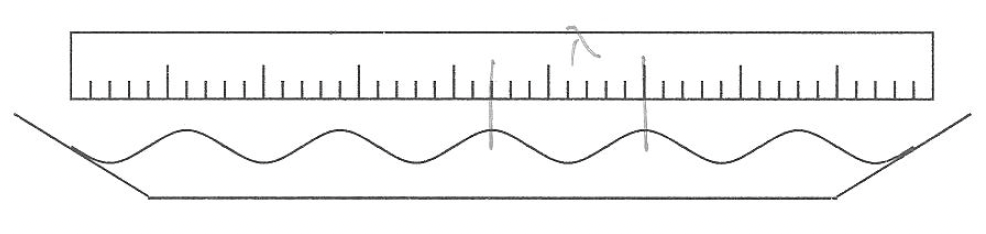
\includegraphics[width=0.75\linewidth]{images/Screenshot 2023-09-26 at 10.12.41 PM.png}
    % \end{figure}
    \par{\par\centering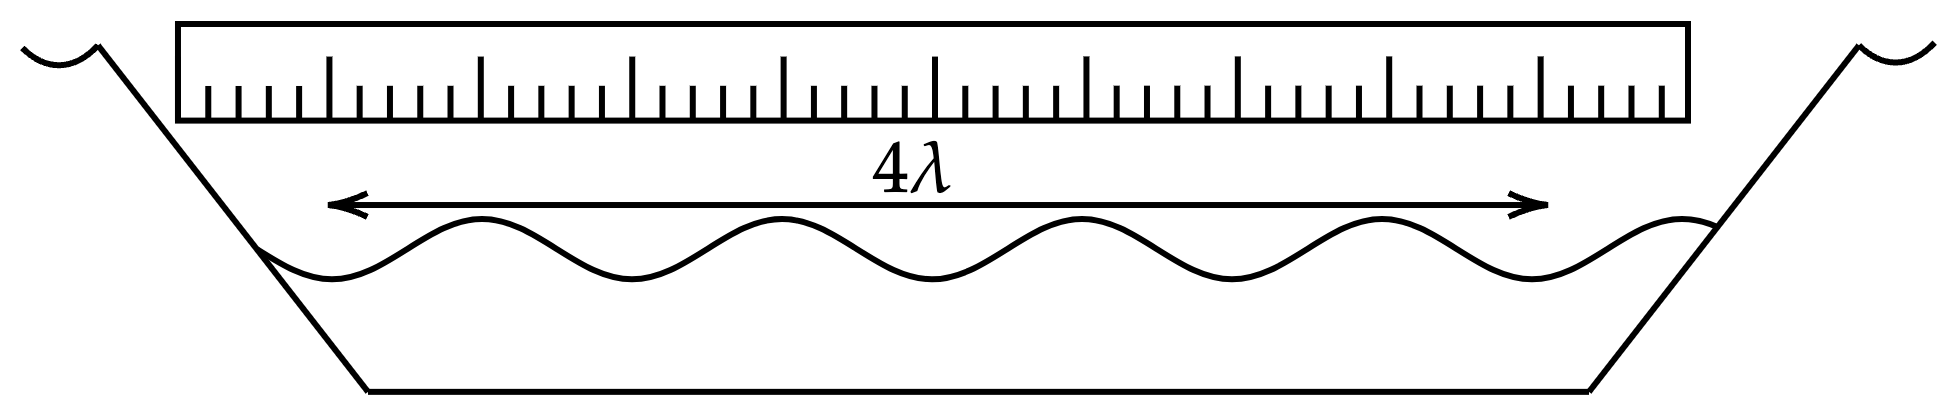
\includegraphics[width=.75\textwidth]{./img/ch2_cf_2024-05-24-13-36-46.png}\par}

\end{frame}
\lecture{Third lecture}{thirdChapter}

\begin{frame}{量度水波的速率Measuring speed of water wave}
    \begin{itemize}
        \item 量度水波槽的兩點距離$d$。\\Measure the distance $d$ between two points in ripple tank.
        \item 使用直振源產生直線波的脈衝。\\Use a vibrating straight bar to generate straight waves.
        \item 使用秒錶量度波傳播$d$的距離所需的時間t。\\Use a stop watch to measure the time $t$ required for the wave to travel a distance $d$.
        \item 水波的速率speed of water wave \(v=\frac{d}{t}\)。
    \end{itemize}\bigskip
\end{frame}

\begin{frame}{水波槽 Ripple tank}
    從牆壁反射的波可能會干擾到觀察的波紋。\\Waves that are reflected from the wall may interfere with the observed wave pattern.
    \begin{itemize}
        \item 減少水波在牆內壁反射:\\To reduce reflection of wave:
    \end{itemize}
    \begin{figure}
        \centering
        % 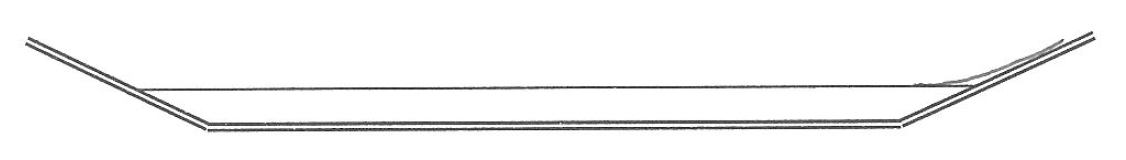
\includegraphics[width=0.75\linewidth]{images/Screenshot 2023-09-26 at 10.23.04 PM.png}
        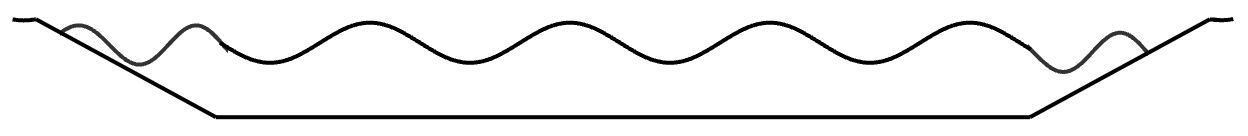
\includegraphics[width=.75\textwidth]{./img/ch2_cf_2024-05-24-13-54-59.png}
        \caption{四邊傾斜 inclined edges}

    \end{figure}
    % \par{\par\centering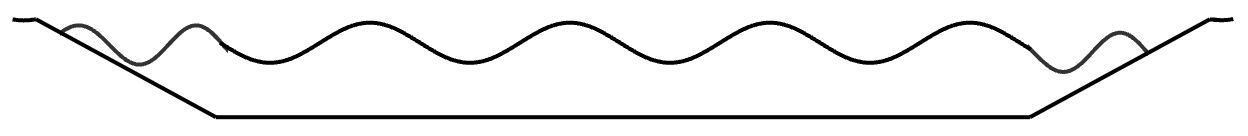
\includegraphics[width=\textwidth]{./img/ch2_cf_2024-05-24-13-54-59.png}\par}
    \begin{figure}
        \centering
        % 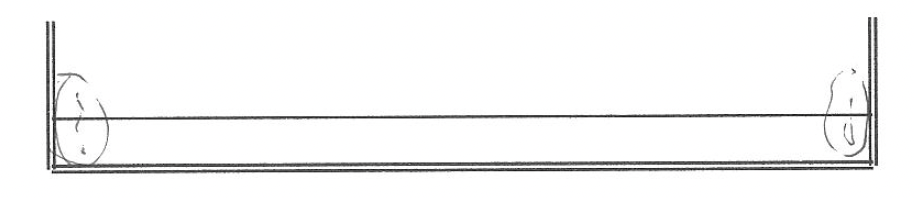
\includegraphics[width=0.7\linewidth]{images/Screenshot 2023-09-26 at 10.23.08 PM.png}
        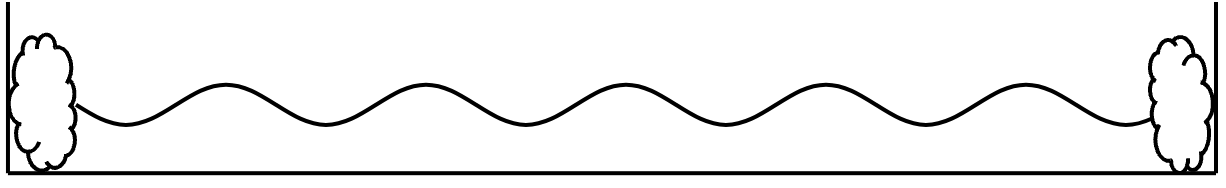
\includegraphics[width=.7\textwidth]{./img/ch2_cf_2024-05-24-13-57-10.png}
        \caption{內壁鋪上海綿 spongy lining}

    \end{figure}
    % \par{\par\centering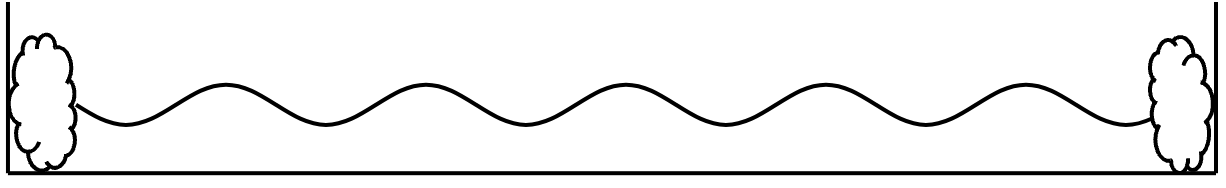
\includegraphics[width=\textwidth]{./img/ch2_cf_2024-05-24-13-57-10.png}\par}
\end{frame}

\begin{frame}{例題Example}
    增加直振源或點振源的振動頻率,對直線波或圓形波會有甚麼影響?\\What is the effect of increasing the frequency of a straight wave or a circular wave?
    \bigskip
    \begin{itemize}
        \item [sol.] 水深不變,波速也不變。\\Water depth is unchanged, wave speed is unchanged.
        \item [] \(v=f\;\lambda\)\
        \item [] $\Rightarrow$頻率 frequency $\uparrow$,波長 wavelength  $\downarrow$。
    \end{itemize}

\end{frame}


\begin{frame}{波的反射現象 Reflection of waves}
    % \begin{figure}
    %     \centering
    %     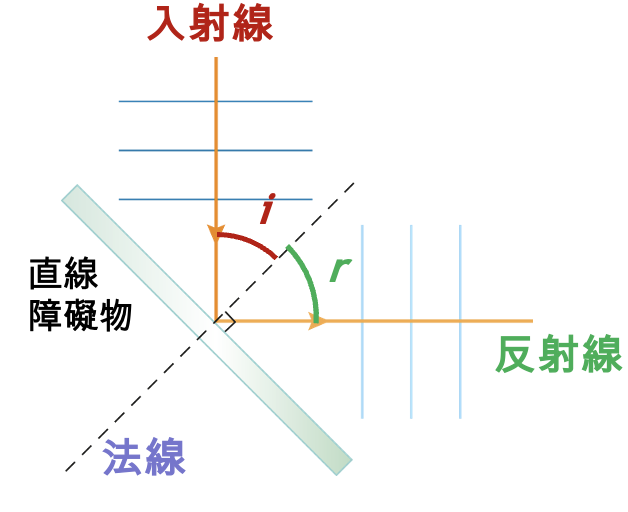
\includegraphics[width=0.5\linewidth]{images/Screenshot 2023-09-26 at 11.31.26 PM.png}


    % \end{figure}
    \par{\par\centering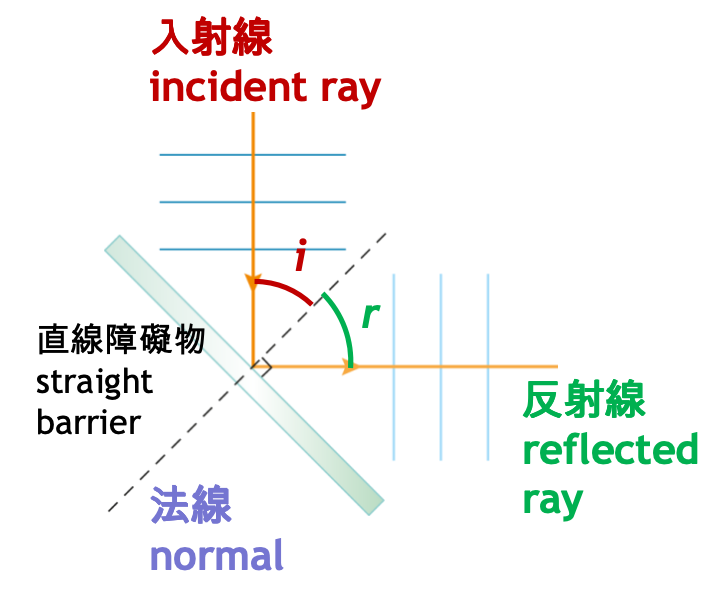
\includegraphics[width=.4\textwidth]{./img/ch2_cf_2024-05-24-14-03-41.png}\par}
    \begin{itemize}
        \item 法線:垂直於反射面的虛構直線\\Normal: constructed line perpendicular to reflecting surface

        \item 入射角 i:入射線和法線之間的夾角\\Angle of incidence i: angle between incident ray and normal
        \item 反射角 r:反射線和法線之間的夾角\\Angle of reflection r: angle between reflected ray and normal
    \end{itemize}
\end{frame}

\begin{frame}{波的反射現象 Reflection of waves}
    \begin{exampleblock}{反射定律 Law of reflection}

        \begin{align*}
            \textrm{反射角 angle of reflection} \;r = \textrm{入射角 angle of incidence} \; i
        \end{align*}
    \end{exampleblock}
    \begin{itemize}
        \item 反射發生在障礙物或邊界。\\Reflection occurs at obstacles or boundaries.
        \item 反射的過程中\\After reflection:
              \begin{itemize}
                  \item 速率、波長、頻率不變。\\speed, wavelength and frequency are unchanged.
                  \item 波的相位可能改變。\\Phase of wave may change.
                  \item 波的傳播方向必定改變。\\Direction of wave is changed.
              \end{itemize}
    \end{itemize}

\end{frame}


\begin{frame}{波的反射現象 Reflection of waves}
    \begin{figure}
        \centering
        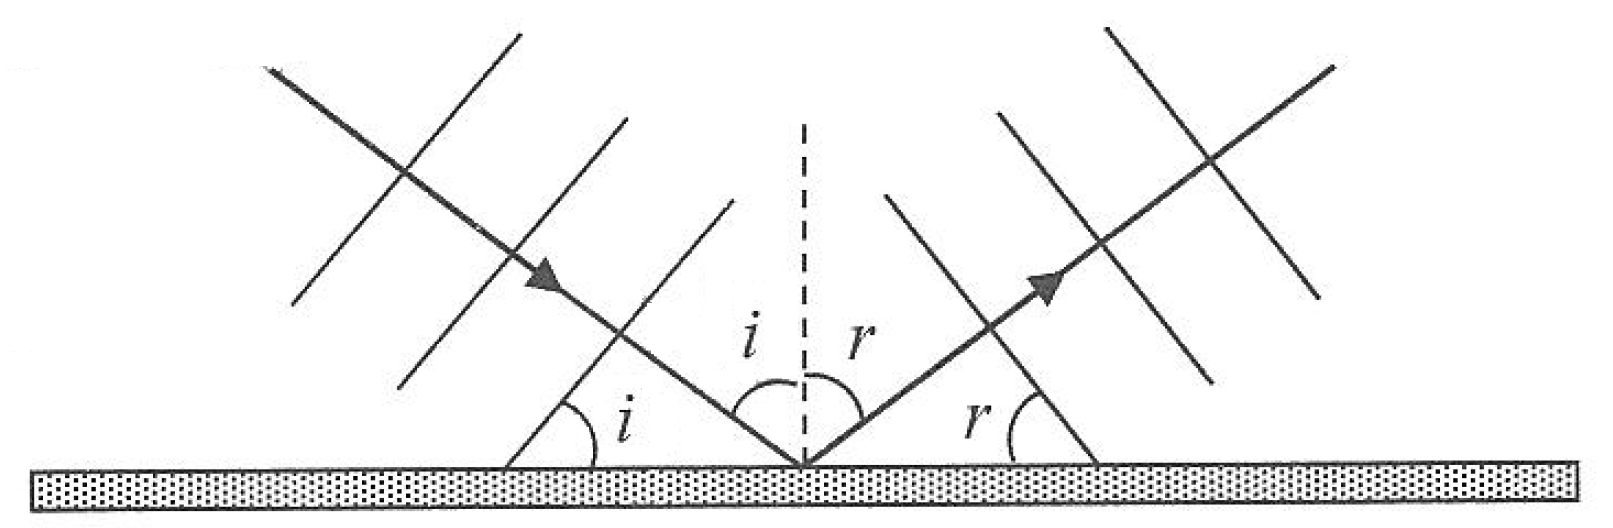
\includegraphics[width=0.5\linewidth]{images/Screenshot_21.png}
    \end{figure}\bigskip
    \begin{figure}
        \centering
        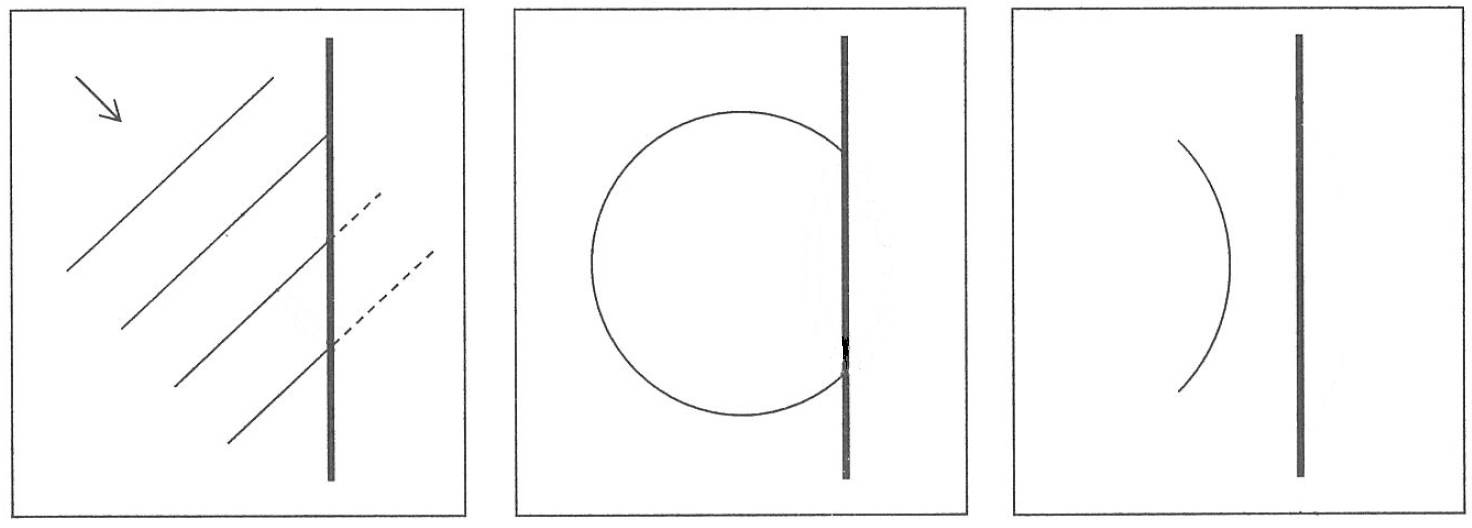
\includegraphics[width=1\linewidth]{images/Screenshot 2023-09-26 at 11.02.18 PM.png}
    \end{figure}
\end{frame}

\begin{frame}[t]{例題Example}
    \begin{figure}
        \centering
        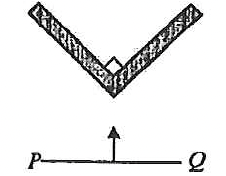
\includegraphics[width=0.25\linewidth]{images/Screenshot 2023-09-27 at 7.20.47 PM.png}


    \end{figure}
    畫出上圖可能的反射脈衝。\\Draw possible reflected pulse.
\end{frame}

\begin{frame}{例題Example}
    \begin{figure}
        \centering
        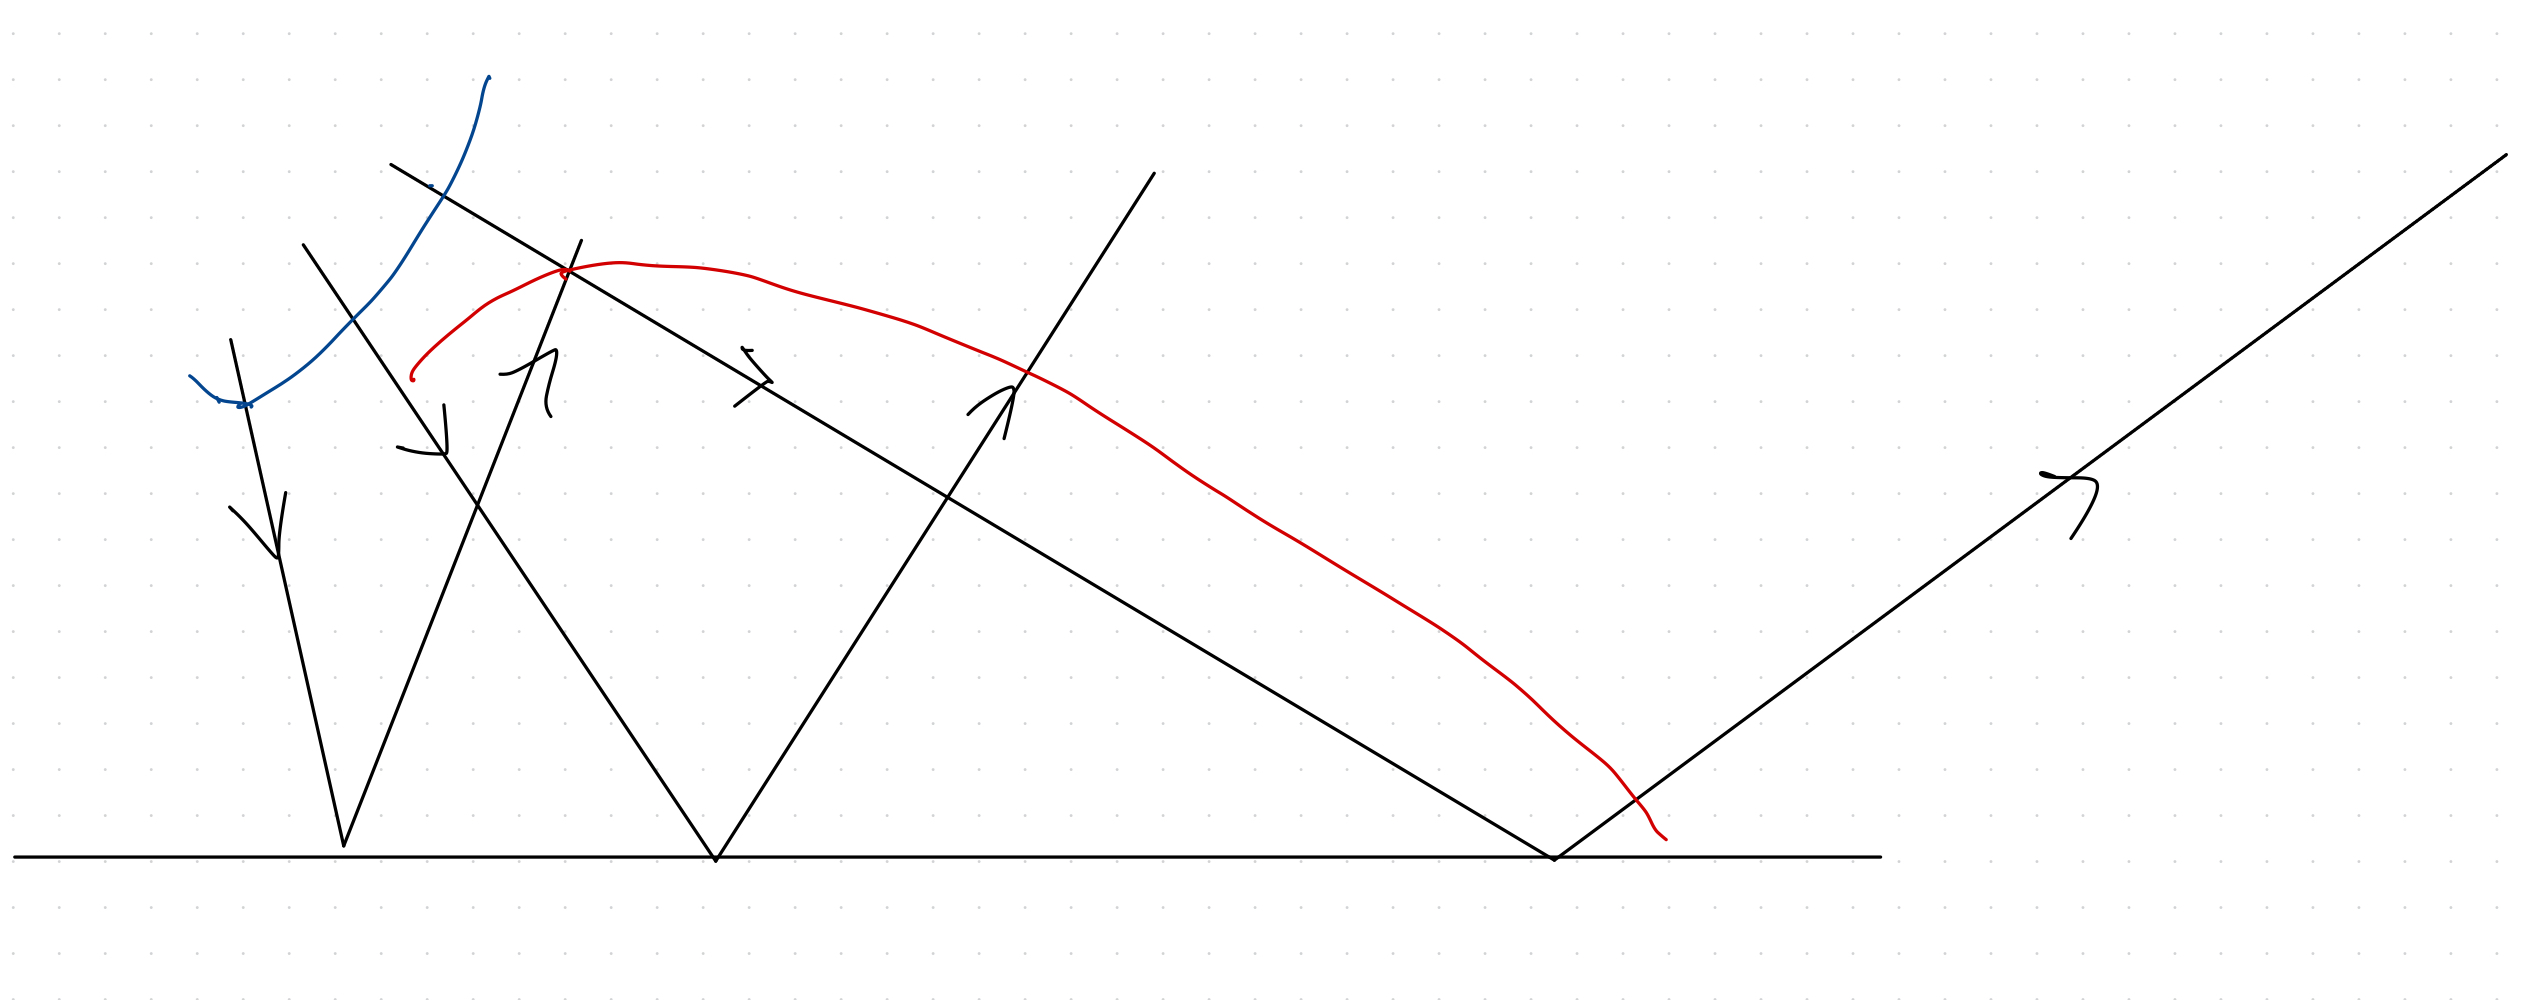
\includegraphics[width=1\linewidth]{images/IMG_F76D36A09E8B-1.jpeg}
    \end{figure}
\end{frame}

\begin{frame}{例題Example}
    \begin{columns}
        \column{.5\textwidth}
        \begin{figure}
            \centering
            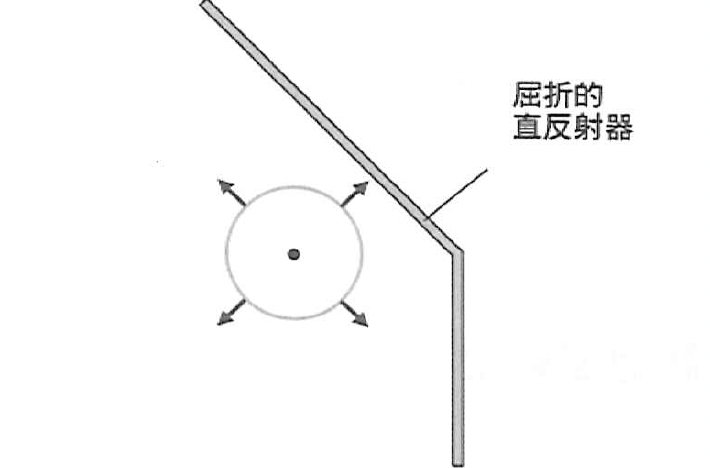
\includegraphics[width=1\linewidth]{images/Screenshot 2023-09-27 at 5.58.33 PM.png}
        \end{figure}
        \column{.5\textwidth}
        \begin{figure}
            \centering
            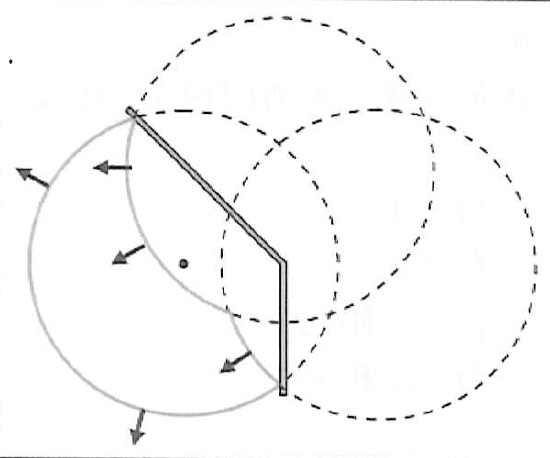
\includegraphics[width=1\linewidth]{images/Screenshot 2023-09-27 at 5.58.44 PM.png}
        \end{figure}
    \end{columns}


\end{frame}

\begin{frame}{例題Example}
    % 水波槽中有兩個相同的正方形方塊。方塊的角相互接觸,且均以一側沿南北方向擺放。一列直線波正以波陣面傾鈄 \qty{45}{^{\circ}} 的方向朝著方塊傳播,如圖所示。以下有關反射波的陳述,哪些是正確的?\\In the water tank, there are two identical square blocks. The corners of the blocks are in contact with each other, and they are placed with one side aligned in the north-south direction. A straight wave is propagating towards the blocks with a wavefront inclined at an angle of \qty{45}{^{\circ}} as shown in the diagram. Which of the following statements about the reflected waves are correct?
    水波槽中有兩個相同的正方形方塊。如圖所示。以下有關反射波的陳述,哪些是正確的?\\In the water tank, there are two identical square blocks. Which of the following statements about the reflected waves are correct?
    \begin{columns}
        \column{.65\textwidth}
        \begin{statements}[before-skip=0.2em,item-indent=3em,label-offset=1em]
            \task 部分反射波沿原路折返。\\Some reflected wave travel back along the same path.
            \task 部分反射波將沿正東方向傳播。\\Some reflected wave travel eastwards.
            \task 這列波將分為三部分,並以不同的方向傳播。\\This wave will be divided into three parts and will propagate in different directions.
        \end{statements}
        \column{.35\textwidth}
        \begin{figure}
            \centering
            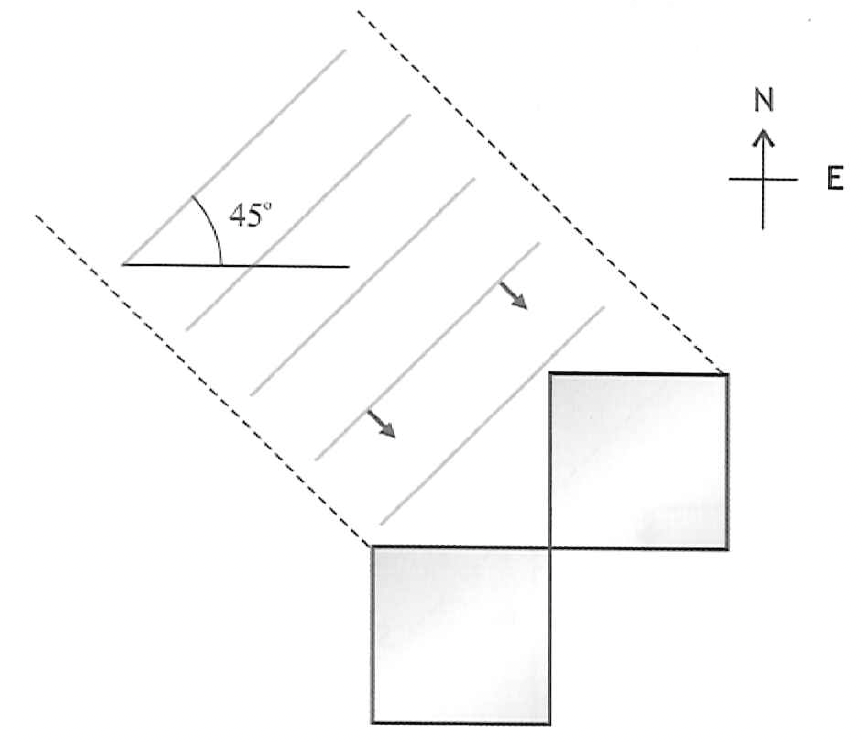
\includegraphics[width=1\linewidth]{images/Screenshot 2023-09-27 at 5.38.43 PM.png}
        \end{figure}
    \end{columns}
\end{frame}



\begin{frame}[t]{例題Example}
    圖中顯示一個直線脈衝正朝著直角反射器傳播。下列哪些是正確的?\\The figure shows a linear pulse propagating towards a right-angle reflector. Which of the following statements are correct?

    \begin{figure}
        \centering
        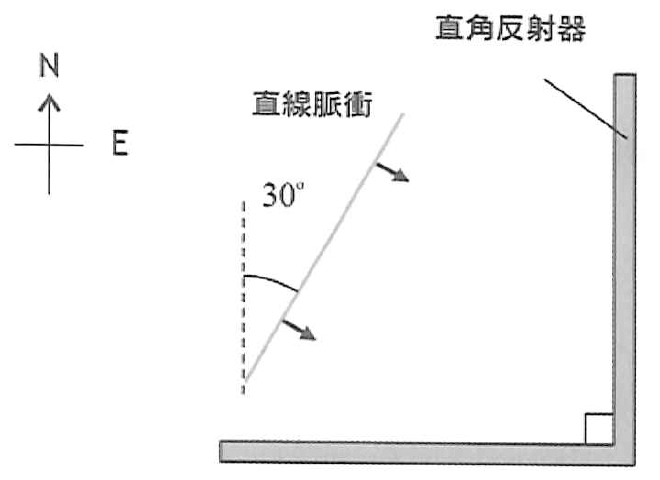
\includegraphics[width=0.6\linewidth]{images/Screenshot 2023-09-27 at 5.37.55 PM.png}
    \end{figure}

\end{frame}

\begin{frame}[t]{例題Example}
    \begin{tasks}
        \task 反射的脈衝將分成兩部分,並以不同的方向離開。\\The reflected pulse will be divided into two parts and will leave in different directions.
        \task 這脈衝將受到反射器的兩面無止境重複的反射。\\The pulse will undergo endless repeated reflections on both sides of the reflector.
        \task 反射脈衝將沿原來的路徑離開反射器。\\The reflected pulse will leave the reflector along its original path.
        \task 在反射過程中,脈衝經過 \dg{60}的旋轉。\\During the reflection process, the pulse undergoes a rotation of \dg{60}.
    \end{tasks}
\end{frame}


\begin{frame}{例題Example}
    一個圓形脈衝遇上直反射器,並已部分進行反射,哪個字母代表反射的部分?\\A circular pulse meets a reflector and has partly reflected. Which letter represents the reflected part of the wave?
    % \begin{figure}
    %     \centering
    %     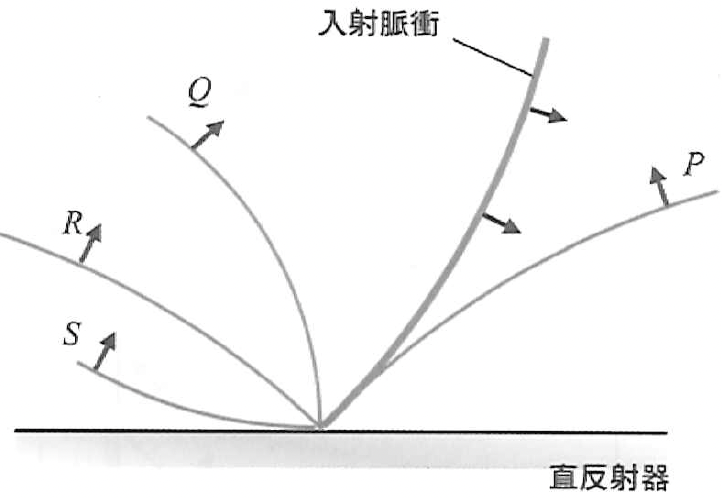
\includegraphics[width=0.5\linewidth]{images/Screenshot 2023-09-27 at 11.19.35 PM.png}
    % \end{figure}
    \par{\par\centering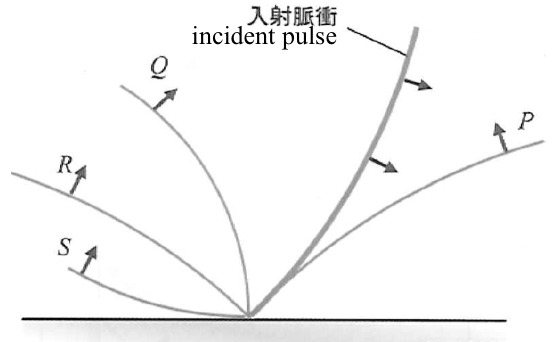
\includegraphics[width=.5\textwidth]{./img/ch2_cf_2024-05-24-14-24-19.png}\par}
    \begin{tasks}(2)[before-skip=0pt]
        \task P
        \task Q
        \task R
        \task S
    \end{tasks}

\end{frame}

% skipped
% \begin{frame}{Rangefinder}
%     \begin{figure}
%         \centering
%         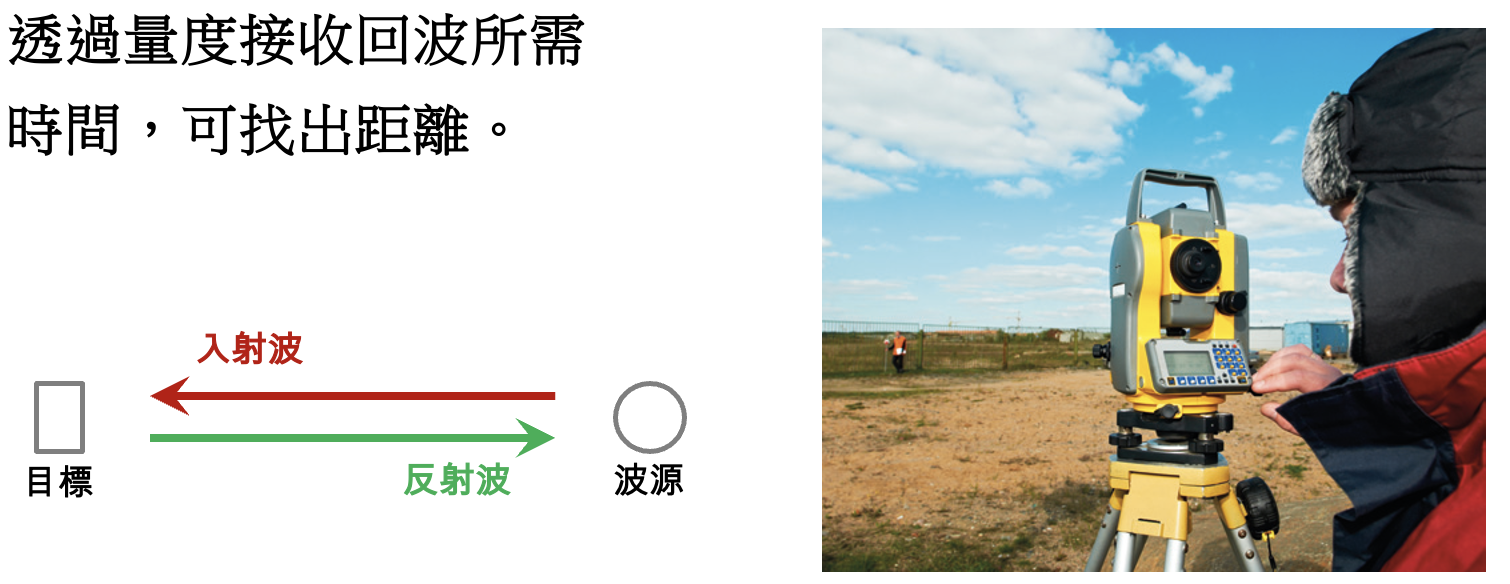
\includegraphics[width=1\linewidth]{images/Screenshot 2023-09-27 at 5.27.30 PM.png}


%     \end{figure}
% \end{frame}




\begin{frame}{反射和相位變化Reflection and phase change}
    \begin{itemize}
        \item 在牆壁上(固定端),反射的波涉及$\pi(180^\circ)$相位改變。\\At the wall (fixed end), the reflected wave involves a phase change of $\pi(180^\circ)$.
    \end{itemize}\bigskip\bigskip
    % \begin{figure}
    %     \centering
    %     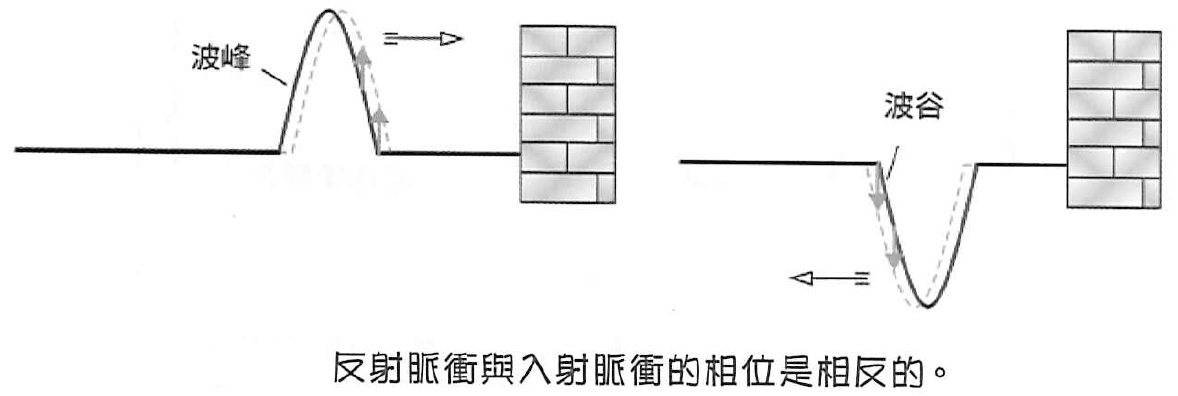
\includegraphics[width=\linewidth]{images/Screenshot 2023-09-27 at 7.11.55 PM.png}
    %     \label{fig:enter-label}
    % \end{figure}
    \par{\par\centering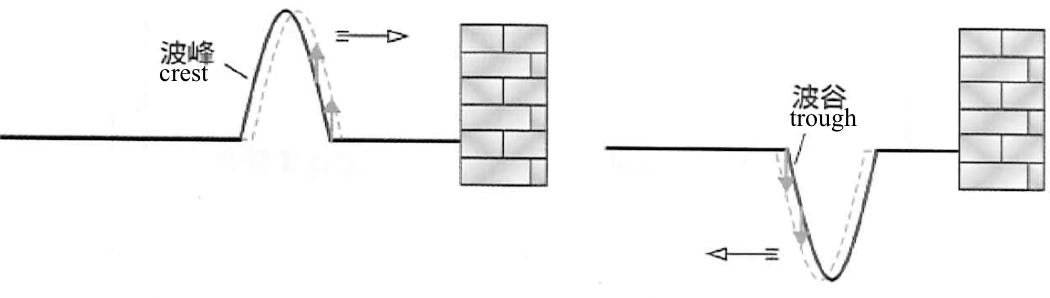
\includegraphics[width=\textwidth]{./img/ch2_cf_2024-05-24-14-26-04.png}\par}
\end{frame}

\begin{frame}{反射和相位變化Reflection and phase change}
    \begin{itemize}
        \item 在自由端,反射的波相位沒有變化。\\At free end, the reflected wave does not involve phase change.
        \item 反射的\textbf{水波}在任何情況下都沒有相位變化。\\Relfected \textbf{water wave} does not have phase change.
    \end{itemize}\bigskip
    % \begin{figure}
    %     \centering
    %     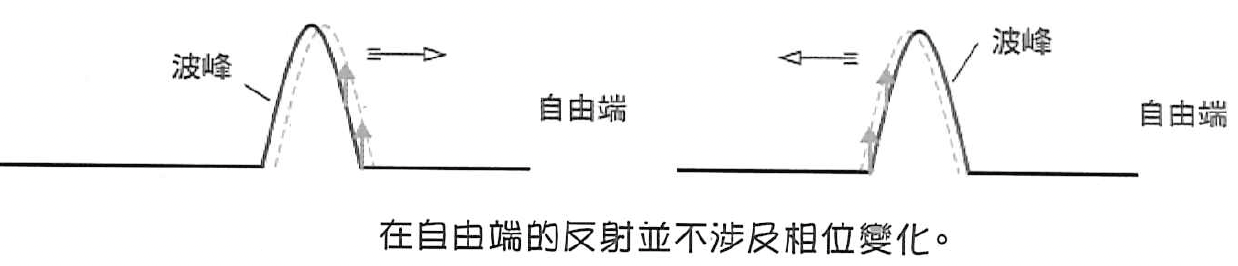
\includegraphics[width=1\linewidth]{images/Screenshot 2023-09-27 at 7.12.02 PM.png}
    % \end{figure}
    \par{\par\centering\includegraphics[width=\textwidth]{./img/ch2_cf_2024-05-24-14-31-18.png}\par}
\end{frame}

\begin{frame}{反射和相位變化Reflection and phase change}
    \begin{figure}
        \centering
        \includegraphics[width=0.75\linewidth]{images/IMG_6F6A16553544-1.jpeg}
        \caption{反射的波形上下左右倒轉 The reflected wave is inverted in both vertical and horizontal directions.}
    \end{figure}
    \begin{figure}
        \centering
        \includegraphics[width=0.75\linewidth]{images/IMG_CBCFA4B99FBF-1.jpeg}
        \caption{反射的波形上下倒轉 The reflected wave is inverted vertically.}
    \end{figure}

\end{frame}



\begin{frame}{折射Refraction of wave}
    \begin{itemize}
        \item
              折射是波動在兩種介質之間傳播時改變方向的現象。\\Refraction is the phenomenon of the change in direction of a wave as it propagates between two different mediums.
    \end{itemize}\bigskip \bigskip
    \begin{figure}
        \centering
        \includegraphics[width=0.75\linewidth]{images/Screenshot 2023-09-27 at 7.33.45 PM.png}
        \caption{左邊是粗繩,右邊是幼繩 Left: thick rope, right: thin rope}
    \end{figure}
\end{frame}

\begin{frame}{折射Refraction of wave}
    在折射的發生時,\\When refraction occurs,
    \begin{itemize}
        \item 頻率不變。 frequency is unchanged.
        \item 波速改變。 wave speed is changed.
        \item 因為\(v=f\lambda\),波長必定改變。 \\\(v=f\lambda\), so wavelength must be changed.
        \item 如果是傾斜進入邊界,波的方向也會改變。 \\Direction of the wave would also change except for normal incidence.
        \item 折射沒有相位改變。 \\ No change in phase.
    \end{itemize}
    % \begin{figure}
    %     \centering
    %     \includegraphics[width=0.75\linewidth]{images/Screenshot 2023-09-27 at 7.42.27 PM.png}
    % \end{figure}
\end{frame}

\begin{frame}{折射Refraction of wave}
    \begin{figure}
        \centering
        \includegraphics[width=0.7\linewidth]{images/Screenshot 2023-09-27 at 7.45.26 PM.png}
        \caption{深水快,淺水慢,$v\propto \lambda$}

    \end{figure}
\end{frame}

\begin{frame}{一個非波例子 A non-wave example}
    \begin{figure}
        \centering
        \includegraphics[width=1\linewidth]{images/Screenshot 2023-09-27 at 9.43.07 PM.png}


    \end{figure}
\end{frame}

\begin{frame}{一個非波例子 A non-wave example}
    \begin{figure}
        \centering
        \includegraphics[width=1\linewidth]{images/Screenshot 2023-09-27 at 9.43.15 PM.png}


    \end{figure}
\end{frame}

\begin{frame}{折射波的方向改變 Direction change of refracted wave}
    \begin{figure}
        \centering
        \includegraphics[width=0.6\linewidth]{images/Screenshot 2023-09-27 at 7.58.53 PM.png}
    \end{figure}
    \begin{alertblock}{波的折射定律 Refraction law of wave}
        \[\frac{\sin \theta_1}{\sin\theta_2}=\frac{v_1}{v_2}=\frac{\lambda_1}{\lambda_2}\]
    \end{alertblock}
\end{frame}
\begin{frame}{折射波的方向改變 Direction change of refracted wave}
    \begin{columns}
        \column{.5\textwidth}
        \begin{figure}
            \centering
            \includegraphics[width=\linewidth]{images/Screenshot 2023-09-27 at 8.51.39 PM.png}


        \end{figure}
        \column{.5\textwidth}
        \begin{figure}
            \centering
            \includegraphics[width=1\linewidth]{images/Screenshot 2023-09-27 at 8.47.44 PM.png}

        \end{figure}
    \end{columns}
    % \begin{figure}
    %     \centering
    %     \includegraphics[width=0.75\linewidth]{images/Screenshot 2023-09-27 at 8.51.39 PM.png}


    % \end{figure}
\end{frame}

\begin{frame}{水波在交界面上的折射 Refraction on boundaries}
    % \begin{figure}
    %     \centering
    %     \includegraphics[width=1\linewidth]{images/Screenshot 2023-09-27 at 8.16.07 PM.png}


    % \end{figure}
    % \par{\par\centering\includegraphics[width=\textwidth]{./img/ch2_cf_2024-05-24-14-42-32.png}\par}
    % \par{\par\centering\includegraphics[width=.6\textwidth]{./img/ch2_cf_2024-05-24-14-51-59.png}\par}
    \par{\par\centering\includegraphics[width=.6\textwidth]{./img/ch2_cf_2024-05-24-14-54-33.png}\par}
\end{frame}
\begin{frame}{水波在交界面上的折射 Refraction on boundaries}
    % \begin{figure}
    %     \centering
    %     \includegraphics[width=1\linewidth]{images/Screenshot 2023-09-27 at 8.16.07 PM.png}


    % \end{figure}
    % \par{\par\centering\includegraphics[width=\textwidth]{./img/ch2_cf_2024-05-24-14-42-32.png}\par}
    \par{\par\centering\includegraphics[width=.6\textwidth]{./img/ch2_cf_2024-05-24-14-52-22.png}\par}
\end{frame}

\begin{frame}{水波在交界面上的折射 Refraction on boundaries}
    \begin{columns}
        \column{.5\textwidth}
        \begin{figure}
            \centering
            \includegraphics[width=1\linewidth]{images/Screenshot 2023-09-27 at 8.28.32 PM.png}


        \end{figure}
        \column{.5\textwidth}
        \begin{figure}
            \centering
            \includegraphics[width=1\linewidth]{images/Screenshot 2023-09-27 at 8.28.43 PM.png}


        \end{figure}
    \end{columns}
\end{frame}

\begin{frame}{水波在交界面上的折射 Refraction on boundaries}
    水波槽中央是一個平凸形狀的淺水區域:\\In the middle of the water tank, there is a shallow region with a flat convex shape.
    \begin{columns}
        \column{.5\textwidth}
        \begin{figure}
            \centering
            \includegraphics[width=1\linewidth]{images/Screenshot 2023-09-27 at 8.31.00 PM.png}


        \end{figure}
        \column{.5\textwidth}
        \begin{figure}
            \centering
            \includegraphics[width=1\linewidth]{images/Screenshot 2023-09-27 at 8.31.30 PM.png}


        \end{figure}
    \end{columns}
\end{frame}

\begin{frame}[t]{例題Example}
    \par{\par\centering\includegraphics[width=\textwidth]{./img/ch2_cf_2024-05-24-15-17-10.png}\par}
\end{frame}

\begin{frame}[t]{例題Example}
    \par{\par\centering\includegraphics[width=\textwidth]{./img/ch2_cf_2024-05-24-15-17-38.png}\par}
\end{frame}

\begin{frame}[t]{例題Example}
    \par{\par\centering\includegraphics[width=\textwidth]{./img/ch2_cf_2024-05-24-15-17-52.png}\par}
\end{frame}

\begin{frame}[t]{例題Example}
    \par{\par\centering\includegraphics[width=\textwidth]{./img/ch2_cf_2024-05-24-15-18-16.png}\par}
\end{frame}


\begin{frame}{水波在交界面上的折射 Refraction on boundaries}

    ...不同於反射,折射時波陣面不會出現「斷折」的情況。\\Unlike reflection, the wavefront cannot possibly `break' during refraction.
    \begin{columns}
        \column{.5\textwidth}
        \begin{figure}
            \centering
            \includegraphics[width=1\linewidth]{images/Screenshot 2023-09-27 at 8.42.42 PM.png}


        \end{figure}
        \column{.5\textwidth}
        \begin{figure}
            \centering
            \includegraphics[width=1\linewidth]{images/Screenshot 2023-09-27 at 8.42.50 PM.png}


        \end{figure}
    \end{columns}
\end{frame}

\begin{frame}{全內反射Total internal reflection}

    從低速介質到高速介質,若入射角持續增加,最終會發生全內反射。\\When the angle of incidence continues to increase from a low-speed medium to a high-speed medium, eventually total internal reflection will occur.
    \bigskip
    \begin{columns}
        \column{.5\textwidth}
        \begin{figure}
            \centering
            \includegraphics[width=1\linewidth]{images/Screenshot 2023-09-27 at 8.56.48 PM.png}


        \end{figure}
        \column{.5\textwidth}
        \begin{figure}
            \centering
            \includegraphics[width=1\linewidth]{images/Screenshot 2023-09-27 at 8.57.33 PM.png}


        \end{figure}
    \end{columns}
\end{frame}

% skipped
% \begin{frame}[t]{例題}
%     試用折射的原理解釋為什麼海灘上的波浪總是平行於岸邊。\medskip
%     \begin{itemize}
%         \item 隨著水波接近岸邊,速率v逐漸減少。
%         \item 行進方向持續彎曲朝向法線,直到與岸邊垂直。
%         \item 所以波陣面平行於岸邊。
%     \end{itemize}
%     \bigskip
%     \begin{columns}
%         \column{.5\textwidth}
%         \begin{figure}
%             \centering
%             \includegraphics[width=\linewidth]{images/Picture1.png}


%         \end{figure}
%         \column{.5\textwidth}
%         \begin{figure}
%             \centering
%             \includegraphics[width=1\linewidth]{images/Picture2.png}


%         \end{figure}
%     \end{columns}
% \end{frame}

\begin{frame}{當繩子遇上繩子(不考)}
    \begin{figure}
        \centering
        \includegraphics[width=0.85\linewidth]{images/Screenshot 2023-09-28 at 10.16.23 AM.png}
        \caption{波進入波密/波疏介質時,出現部分反射,部分折射的現象}

    \end{figure}
\end{frame}

\begin{frame}{衍射(繞射) Diffraction}
    \begin{itemize}
        \item 當行波經過狹縫或阻礙物邊緣時,會發生衍射,擴散至狹縫或阻礙物後方的區域。\\When a wave passes through a narrow gap or encounters the edge of an obstacle, diffraction occurs, spreading into the region behind the gap or obstacle.

    \end{itemize}
    \begin{figure}
        \centering
        \includegraphics[width=1\linewidth]{images/Screenshot 2023-09-27 at 9.46.49 PM.png}


    \end{figure}
\end{frame}

\begin{frame}
    \frametitle{衍射(繞射) Diffraction}
    \begin{itemize}
        \item 衍射過程中 For diffraction:
              \begin{itemize}
                  \item 速率、頻率和波長都不會改變。\\ speed, frequency and wavelength do not change.
                  \item 只會改變波在障礙物邊緣的傳播方向。\\only the direction of wave propagation at the edges of obstacles will change.
              \end{itemize}
        \item 衍射是波獨有的現象。可以用這現象來判斷一個事物是不是波。\\Diffraction is unique to waves, and it can be a reason to show that something is wave-like.
    \end{itemize}

\end{frame}

\begin{frame}{衍射Diffraction}
    \begin{figure}
        \centering
        \includegraphics[width=1\linewidth]{images/Screenshot 2023-09-27 at 9.09.03 PM.png}


    \end{figure}
\end{frame}

\begin{frame}[t]{例題Example}

\end{frame}

\begin{frame}[t]{例題Example}

\end{frame}


\begin{frame}{影響衍射程度的因素 Factors affecting extent of diffraction}
    \begin{itemize}
        \item 衍射的程度是根據$\displaystyle \frac{\lambda}{\texttt{a}}$影響。\\The extent of diffraction $\sim\displaystyle \frac{\lambda}{\texttt{a}}$
              \begin{itemize}
                  \item 波長$\uparrow\ \Rightarrow$衍射程度$\uparrow$
                  \item 狹縫寬度$\uparrow\ \Rightarrow$衍射程度$\downarrow$
              \end{itemize}
        \item 阻礙物的大小不影響衍射的程度,除非障礙物極小至能讓波直接穿過。
        \item 圓形波:\(\lambda \approx a\)
        \item 振幅減半:$\lambda \approx 2a$
    \end{itemize}
\end{frame}

\begin{frame}{不同縫隙寬度的衍射 Diffraction for different gap width}
    \begin{figure}
        \centering
        \includegraphics[width=0.95\linewidth]{images/Screenshot 2023-09-27 at 9.51.08 PM.png}


    \end{figure}
\end{frame}

\begin{frame}{不同波長的衍射 Diffraction for different wavelengths}
    \begin{figure}
        \centering
        \includegraphics[width=0.95\linewidth]{images/Screenshot 2023-09-27 at 9.50.14 PM.png}


    \end{figure}
\end{frame}
\begin{frame}{例題}
    水波槽中,一道屏障中央有一個縫隙。以下哪些改變可增加平面水波穿過該縫隙時的繞射程度?\\In the water tank, there is a gap in the center of a barrier. Which of the following changes can increase the degree of diffraction when a plane water wave passes through the gap?

    \begin{statements}
        \task 增加振動頻率。\\Increase frequency of oscillation.
        \task 減少水深。\\Decrease depth of water.
        \task 減少縫隙的寬度。\\Increase width of the gap.
    \end{statements}

    % \begin{mchoices}
    %     \begin{mmc}
    %         \item 只有(1)
    %         \item 只有(3)
    %     \end{mmc}
    %     \begin{mmc}
    %         \item 只有(1)和(2)
    %         \item 只有(2)和(3)
    %     \end{mmc}
    % \end{mchoices}

    % \begin{mmchoices}
    %     \item 只有(1)
    %     \item 只有(3)
    %     \item 只有(1)和(2)
    %     \item 只有(2)和(3)
    % \end{mmchoices}
\end{frame}

\end{document}